\documentclass[10pt,a4paper]{article}
\usepackage{amssymb} %mathbb
\usepackage{amsmath} %align
\usepackage{eucal}
\usepackage{hyperref}
\usepackage{cancel}
\usepackage{array,bm}
\usepackage{graphicx} %jpg
\usepackage{tikz-cd}
\usetikzlibrary{arrows, matrix}
\usepackage[top=1.0cm,bottom=1.3cm,left=1.0cm,right=1.0cm]{geometry}
\newcolumntype{C}{>{$}c<{$}}
\renewcommand{\arraystretch}{1.2}
\begin{document}
	\Large

	\begin{center}
		Lista de Geometria de Riemann, Vin\'icius Claudino Ferraz, 01/11/2018
	\end{center}

	\normalsize

Tensorial Video on \href{https://www.youtube.com/watch?v=mmzqmIcX7xo}{\color{blue}\underline{YouTube}}. Riemannian Geometry Video on \href{https://www.youtube.com/watch?v=Z3IXeWvEEa4}{\color{blue}\underline{YouTube}}.

	\section{Quest\~ao de Lee 4.1}
		\begin{flushright}
		\end{flushright}

		Sejam $M, \nabla$ e as bases ortonormais locais $\{ \partial_i \}, \{ \overline{\partial}_j \}$ em $U$ aberto contido em $M$. Relacionados por $\overline{\partial}_i = A_{ij} \partial_j$, em que $A$ \'e matriz.

		Sejam $\Gamma_{ij}^k, \overline{\Gamma}_{ij}^k$ os s\'imbolos de Christoffel com respeito a ambas as frames. Encontre a transforma\c{c}\~ao $(\overline{\Gamma}_{ij}^k, A_{ij}) \mapsto \Gamma_{ij}^k$.

		\vspace{12mm}

		Pela equa\c{c}\~ao 3.2:

		\begin{align*}
  		\nabla_{\partial_i} \partial_j &= \sum_k \overline{\Gamma}_{ij}^k \overline{\partial}_k, \forall i, j \in \{ 1, 2, \cdots, n \} \\
  		\nabla_{\partial_i} \partial_j &= \sum_k \Gamma_{ij}^k \partial_k, \forall i, j \\
		\sum_k \overline{\Gamma}_{ij}^k \bigg(\sum_\ell A_{k\ell} \partial_\ell \bigg) &= \sum_\ell \Gamma_{ij}^\ell \partial_\ell, \forall i, j \\
		\sum_k \overline{\Gamma}_{ij}^k A_{k\ell} &= \Gamma_{ij}^\ell, \forall i, j, \ell \\
		\left(\begin{matrix} \overline{\Gamma}_{ij}^1 & \cdots & \overline{\Gamma}_{ij}^n \end{matrix}\right) \cdot \text{col}_k(A) &= \Gamma_{ij}^k, \forall i, j, k
		\end{align*}

		S\~ao $n^3$ igualdades, porque $1 \le k \le n$.

		\vspace{12mm}

	\section{Quest\~ao 2}
		\begin{flushright}
		\end{flushright}

		\textbf{Modelo do hiperboloide de duas folhas}

		Espa\c{c}o $\mathcal{H}^2 = \{ (\xi, \sigma, \tau) \in \mathbb{R}^3 \,; \tau > 0 \,; \tau^2 - \xi^2 - \sigma^2 = 1 \}$

		M\'etrica $g^1 = i^* m'$, em que $i : \mathcal{H}^2 \rightarrow \mathbb{R}^3$ \'e a inclus\~ao e	$m' = \sum \sum m_{ij}\, \mathrm{d}x^i \otimes \mathrm{d}x^j \Rightarrow M' = \left( \begin{matrix} 1 & 0 & 0 \\ 0 & 1 & 0 \\ 0 & 0 & -1 \end{matrix} \right)$

		Usando a equa\c{c}\~ao 2.6 (Produto sim\'etrico de tensores)

		\vspace{6mm}

		\textbf{Modelo do disco de Poincar\'e}

		Espa\c{c}o $B^2 = \{ (u, v) \in \mathbb{R}^2 \,; u^2 + v^2 < 1 \}$ com a m\'etrica $G^2 = \cfrac{4}{(1 - u^2 - v^2)^2} \left( \begin{matrix} 1 & 0 \\ 0 & 1 \end{matrix} \right)$.

		\vspace{6mm}

		\textbf{Modelo do semiplano de Poincar\'e}

		Espa\c{c}o $\mathbb{H}^2 = \{ (x,y) \in \mathbb{R}^2 \,; y > 0 \}$ com a m\'etrica $G^3 = \cfrac{1}{y^2} \left( \begin{matrix} 1 & 0 \\ 0 & 1 \end{matrix} \right)$.

		\vspace{6mm}

		Isometrias

		\[
		\begin{tikzcd}
		                                              & \mathcal{H}^2 \arrow{r}{\kappa \circ \pi} & \mathbb{H}^2  \\
		\mathcal{H}^2 \arrow{ur}{\Psi} \arrow{r}{\pi} & B^2 \arrow{r}{\kappa}                     & \mathbb{H}^2 \arrow{u}{T}  \\
		                                              & S^2 \arrow{r}{f} \arrow{u}{\omega}        & S^2 \arrow{u}{\omega}
		\end{tikzcd}
		\]

		$\pi$ \'e difeomorfismo, proje\c{c}\~ao estereogr\'afica hiperb\'olica.

		Seja $S = (0,0,-1) \in \mathbb{R}^3$. Para cada $P = (\xi, \sigma, \tau) \in \mathcal{H}^2$, associamos $\pi(P) = U \in B^2$, em que $U = (u, v) \in \mathbb{R}^2$ \'e o ponto de interse\c{c}\~ao da reta $SP$ com o plano $\{ \tau = 0 \}$.

		Temos $U - S = \lambda (P - S)$, para algum $\lambda \in \mathbb{R}$.

		\begin{equation*}
			\left.\begin{aligned}
			    u &= \lambda \xi \\
			    v &= \lambda \sigma \\
			    1 &= \lambda (\tau + 1)
			\end{aligned}
			\right\} \Rightarrow \pi(\xi, \sigma, \tau) = (u, v) = \cfrac{1}{1 + \tau} \cdot (\xi, \sigma)
		\end{equation*}

		$\pi^{-1}(u, v) = (\xi, \sigma, \tau) = \bigg( \cfrac{2}{1 - u^2 - v^2} \cdot u \,; \cfrac{2}{1 - u^2 - v^2} \cdot v \,; \cfrac{1 + u^2 + v^2}{1 - u^2 - v^2} \bigg)$ [verificado]

		Defini\c{c}\~ao de Lee, p. 24: $(M, g^1)$ e $(N, g^2)$ s\~ao variedades riemannianas. Um difeo $\varphi: M \rightarrow N$ \'e isometria se $\varphi^* g^2 = g^1$.

		\subsection{Verificar que ${(\pi^{-1})}^* g^1 = g^2$}

		\begin{flushright}
		\end{flushright}

		Seja $V \in T_{(u, v)}B^2$. Lee denota no fim da p. 36: $\pi^{-1}_* V = V\xi \partial_{\xi} + V\sigma \partial_{\sigma} + V\tau \partial_\tau$.

		\begin{align*}
		{(\pi^{-1})}^* g^1(V,V) &= g^1(\pi^{-1}_* V, \pi^{-1}_* V) \text{ (Por qu\^e? Neste ponto engaveto o arquivo, sem saber.)} \\
		&= \langle \pi^{-1}_* V, \pi^{-1}_* V\rangle_{(\xi, \sigma, \tau)} = (V\xi)^2 + (V\sigma)^2 - (V\tau)^2 \\
		V\xi &= \sum_i V^i \partial_i \xi = V^1 \cdot \cfrac{\partial \xi}{\partial u} + V^2 \cdot \cfrac{\partial \xi}{\partial v} \Rightarrow V\sigma = V^1 \cdot \cfrac{\partial \sigma}{\partial u} + V^2 \cdot \cfrac{\partial \sigma}{\partial v} \Rightarrow V\tau = V^1 \cdot \cfrac{\partial \tau}{\partial u} + V^2 \cdot \cfrac{\partial \tau}{\partial v} \\
		\theta(u, v) &= (1 - u^2 - v^2)^2 \\
		J\pi^{-1} &= \left[ \begin{matrix} \xi_u & \xi_v \\ \sigma_u & \sigma_v \\ \tau_u & \tau_v \end{matrix} \right] = \left[ \begin{matrix} \frac{2 + 2u^2 - 2v^2}{\theta} & \frac{4uv}{\theta} \\ \frac{4uv}{\theta} & \frac{2 - 2u^2 + 2v^2}{\theta} \\ \frac{4u}{\theta} & \frac{4v}{\theta} \end{matrix} \right] \ne 0 \\
		{(\pi^{-1})}^* g^1(V,V) &= \bigg(V^1 \cdot \cfrac{2 + 2u^2 - 2v^2}{\theta} + V^2 \cdot \cfrac{4uv}{\theta}\bigg)^2 + \bigg(V^1 \cdot \cfrac{4uv}{\theta} + V^2 \cdot \cfrac{2 - 2u^2 + 2v^2}{\theta} \bigg)^2 - \bigg(V^1 \cdot \cfrac{4u}{\theta} + V^2 \cdot \cfrac{4v}{\theta} \bigg)^2 \\
	  &= \cfrac{4}{\theta^2} \cdot (A V^1 V^1 + C V^1 V^2 + K V^2 V^2) = g^2(V, V) = \langle V, V \rangle_{(u,v)} = 4 \cdot \cfrac{V^1 V^1 + V^2 V^2}{\theta} \\
		A &= (1 + u^2 - v^2)^2 + 4 u^2 v^2 - 4u^2 \\
		C &= 2 [(1 + u^2 - v^2)2uv + 2uv(1-u^2+v^2) - 4uv] \\
		K &= 4u^2v^2 + (1 - u^2 + v^2)^2 - 4v^2 \\
		&\text{Queremos mostrar que } A = \theta, C = 0, K = \theta \\
		\theta &= 1 + u^4 + v^4 - 2u^2 - 2v^2 + 2u^2 v^2 = 1 + u^4 + v^4 + 2u^2 - 2v^2 - 2u^2 v^2 + 4 u^2 v^2 - 4u^2, \forall (u,v) \in B \\
		0 &= C \Rightarrow u = 0 \vee v = 0 \vee 0 = 0\cdot u^2, \forall (u,v) \in B \\
		\theta &= 1 + u^4 + v^4 - 2u^2 - 2v^2 + 2u^2 v^2 = 4u^2 v^2 + 1 + u^4 + v^4 - 2u^2 + 2v^2 - 2u^2 v^2 - 4 v^2, \forall (u,v) \in B^2\,\,\blacksquare
		\end{align*}

		\vspace{3mm}

		Caso $V \ne W \in T_{(u,v)}B^2$:

		\begin{align*}
		{(\pi^{-1})}^* g^1(V + W, V + W) &= g^1(\pi^{-1}_* (V + W), \pi^{-1}_* (V + W)) = \\
		= \langle \pi_*^{-1} (V + W), \pi_*^{-1} (V + W) \rangle_P &= \langle \pi_*^{-1} V, \pi_*^{-1} V \rangle_P + 2 \langle \pi_*^{-1} V, \pi_*^{-1} W \rangle_P + \langle \pi_*^{-1} W, \pi_*^{-1} W \rangle_P \\
		g^2(V + W, V + W) &= \langle V + W, V + W \rangle_{(u,v)} = \langle V, V \rangle_{(u,v)} + 2 \langle V, W \rangle_{(u,v)} + \langle W, W \rangle_{(u,v)} \\
		\Rightarrow 2 \langle \pi_*^{-1} V, \pi_*^{-1} W \rangle_P &= 2 \langle V, W \rangle_{(u,v)} \\
		\therefore {(\pi^{-1})}^* g^1(V, W) &= g^2(V, W)
		\end{align*}

		\vspace{3mm}

		$\kappa$ \'e difeomorfismo, transformada de Cayley.

		Sejam $(u, v) \in B^2\,; w = u + vi\,; z = x + yi\,; (x, y) \in \mathbb{H}^2$.

		$\kappa(w) = z = -i \cdot \cfrac{w + i}{w - i} \Rightarrow \kappa(u,v) = (x,y) = \bigg( \cfrac{2u}{u^2 + (v-1)^2} \,; \cfrac{1 - u^2 - v^2}{u^2 + (v-1)^2}  \bigg)$ [ok]

		$\kappa^{-1}(x,y) = (u,v) = \bigg( \cfrac{2x}{x^2 + (y+1)^2} \,; \cfrac{x^2 + y^2 - 1}{x^2 + (y+1)^2}  \bigg)$ [ok]

		\vspace{120mm}

		\subsection{Provar que $\kappa^* g^3 = g^2$}

		\begin{flushright}
		\end{flushright}

		Seja $V \in T_{(u,v)}B^2$. Lee denota no fim da p. 36: $\kappa_* V = Vx \partial_x + Vy \partial_y$.

		\begin{align*}
		\kappa^* g^3(V,V) &= g^3(\kappa_* V, \kappa_* V) \\
		&= \langle \kappa_* V, \kappa_* V\rangle_{(x,y)} = \cfrac{1}{y^2} \cdot [(Vx)^2 + (Vy)^2] \\
		Vx &= \sum_i V^i \partial_i x = V^1 \cdot \cfrac{\partial x}{\partial u} + V^2 \cdot \cfrac{\partial x}{\partial v} \Rightarrow Vy = V^1 \cdot \cfrac{\partial y}{\partial u} + V^2 \cdot \cfrac{\partial y}{\partial v} \\
		\gamma(u,v) &= [u^2 + (v-1)^2]^2
		\end{align*}

		\begin{align*}
		J\kappa &= \left[ \begin{matrix} x_u & x_v \\ y_u & y_v \end{matrix} \right] = \left[ \begin{matrix} \cfrac{2(v-1)^2 - 2u^2}{\gamma} & \cfrac{-4u(v-1)}{\gamma} \\ -2u \cdot \cfrac{-2v + 2}{\gamma} & 2 \cdot \cfrac{(v - 1)^2 - u^2}{\gamma} \end{matrix} \right] = 0, \text{ se } (u,v) = (0,1) \notin B^2 \\
		\kappa^* g^3(V,V) &= \cfrac{\gamma}{(1 - u^2 - v^2)^2} \bigg[\bigg(V^1 \cfrac{2(v-1)^2 - 2u^2}{\gamma} + V^2 \cfrac{-4u(v-1)}{\gamma}\bigg)^2 + \bigg(V^1 \cfrac{4uv - 4u}{\gamma} + V^2 \cfrac{2(v - 1)^2 - 2u^2}{\gamma}\bigg)^2\bigg] \\
		&= \cfrac{\{V^1 \cdot [2(v-1)^2 - 2u^2] - V^2 \cdot 4u(v-1)\}^2 + \{V^1 \cdot (4uv - 4u) + V^2 \cdot [2(v-1)^2 - 2u^2]\}^2}{\gamma(1 - u^2 - v^2)^2} \\
		&= \cfrac{A V^1 V^1 + C V^1 V^2 + K V^2 V^2}{\gamma(1 - u^2 - v^2)^2} =	g^2(V,V) = \langle V, V\rangle_{(u,v)} = \cfrac{4}{(1 - u^2 - v^2)^2} \cdot (V^1 V^1 + V^2 V^2) \\
		A &= [2(v-1)^2 - 2u^2]^2 + (4uv - 4u)^2 \\
		C &= - 2 [2(v-1)^2 - 2u^2] \cdot 4u(v-1) + 2 (4uv - 4u) \cdot [2(v-1)^2 - 2u^2] \\
		K &= 16u^2(v-1)^2 + 4[(v - 1)^2 - u^2]^2 \\
		&\text{Queremos mostrar que } \cfrac{A}{\gamma} = 4, C = 0, \cfrac{K}{\gamma} = 4 \\
		[u^2 + (v-1)^2]^2 &= [(v-1)^2 - u^2]^2 + 4(uv - u)^2 \Rightarrow 4 u^2 (v-1)^2 = 4(uv - u)^2 \Rightarrow u = 0 \vee 0\cdot v = 0, \forall (u, v) \in B^2 \\
		0 &= - [(v-1)^2 - u^2] \cdot u(v-1) + (uv - u) \cdot (v^2 - 2v + 1 - u^2) \\
		\Rightarrow u &= 0 \vee v - 1 = 0 \vee (v-1)^2 =  v^2 - 2v + 1, \forall (u,v) \in B^2 \\
		[u^2 + (v-1)^2]^2 &= 4u^2(v-1)^2 + [(v- 1)^2 - u^2]^2 \\
		\Rightarrow &\cancel{u^4} + 2 u^2 (v-1)^2 + \cancel{(v-1)^4} = 4u^2(v-1)^2 + \cancel{(v- 1)^4} - 2 (v-1)^2 u^2 + \cancel{u^4}, \forall (u,v) \in B^2 \,\,\blacksquare
		\end{align*}

		\subsection{Exerc\'icio de Lee 3.11 na p. 41}
		\begin{flushright}
		\end{flushright}

		Provar que $\kappa = \omega \circ f \circ \omega^{-1}$.

		$f : S^2 \rightarrow S^2$ \'e rota\c{c}\~ao. $f(x,y,z) = (x, -z, y) \Rightarrow f(\{z < 0\}) = \{y > 0\} \subset S^2$. Isso evita o polo Norte.

		$\omega : S^2 - \{ N \} \rightarrow \mathbb{R}^2$ \'e proje\c{c}\~ao estereogr\'afica. $\omega(x,y,z) = (u,v) = \cfrac{1}{1-z} \cdot (x, y)$

		$\Rightarrow \omega^{-1}(u, v) = (x, y, z) = \bigg( \cfrac{2u}{u^2 + v^2 + 1}, \cfrac{2v}{u^2 + v^2 + 1}, \cfrac{u^2 + v^2 - 1}{u^2 + v^2 + 1} \bigg) \Rightarrow z < 0$

		$\Rightarrow (f \circ \omega^{-1})(u, v) = (x', y', z') = \bigg( \cfrac{2u}{u^2 + v^2 + 1}, \cfrac{1 - u^2 - v^2}{u^2 + v^2 + 1}, \cfrac{2v}{u^2 + v^2 + 1} \bigg)$

		$\Rightarrow (\omega \circ f \circ \omega^{-1})(u, v) = (u', v') = \cfrac{1}{1-\cfrac{2v}{u^2 + v^2 + 1}} \cdot \bigg( \cfrac{2u}{u^2 + v^2 + 1}, \cfrac{1 - u^2 - v^2}{u^2 + v^2 + 1} \bigg) = \kappa(u, v) \therefore \omega \circ f \circ \omega^{-1} \bigg\vert_{B^2} = \kappa\,\,\blacksquare$

		\subsection{Calcular o pullback na forma complexa $z = \kappa(w)$}
		\begin{flushright}
		\end{flushright}

		$\kappa(w) = z = -i \cdot \cfrac{w + i}{w - i} \Rightarrow \kappa_w(w) = -i \cdot \cfrac{w - i - w - i}{(w - i)^2}= \cfrac{-2}{(w - i)^2} \Rightarrow g^2 = \cfrac{4\, \mathrm{d}w \, \mathrm{d}\overline{w}}{(1 - \vert w \vert^2)^2} \Rightarrow g^3 = \cfrac{\mathrm{d}z \, \mathrm{d}\overline{z}}{(\text{Im } z)^2}$

		Utilize que $\kappa^* (\mathrm{d}z \, \mathrm{d}\overline{z}) = \vert \kappa_w(w) \vert^2 \, \mathrm{d}w \, \mathrm{d}\overline{w}$. (Essa tamb\'em vai ficar pra pr\'oxima.)

		$\kappa^* g^3 = \kappa^* \cfrac{\mathrm{d}z \, \mathrm{d}\overline{z}}{(\text{Im } z)^2} = \cfrac{1}{(\text{Im } z)^2} \cdot \kappa^* (\mathrm{d}z \, \mathrm{d}\overline{z}) = \cfrac{1}{(\text{Im } z)^2} \cdot \vert \kappa_w(w) \vert^2 \, \mathrm{d}w \, \mathrm{d}\overline{w} = g^2 = \cfrac{4\, \mathrm{d}w \, \mathrm{d}\overline{w}}{(1 - \vert w \vert^2)^2}$

		$\Rightarrow \cfrac{1}{(\text{Im } z)^2} \cdot \bigg\vert \cfrac{-2}{(w - i)^2} \bigg\vert^2 = \cfrac{4}{(1 - \vert w \vert^2)^2} \Rightarrow (\text{Im } z)^2 \cdot \vert (w - i)^2 \vert^2 = (1 - \vert w \vert^2)^2 \Rightarrow (\text{Im } z) \cdot \vert (w - i)^2 \vert = \epsilon (1 - \vert w \vert^2)$

		$w \in B^2 \therefore 0 < \text{Im } k(w) = + \cfrac{1 - \vert w \vert^2}{\vert w - i \vert^2}$, Q. E. D. $\,\,\blacksquare$

		\subsection{Seja $n \ge 3$}
		\begin{flushright}
		\end{flushright}

		O c\'alculo de $g^3 (\kappa_* V, \kappa_* V)$ se reduz ao caso 2D, conjugando $\kappa$ com uma transforma\c{c}\~ao ortogonal em $n - 1$ vari\'aveis.

		Seja $\kappa^2(u, v, x_3, \cdots, x_n) = (x, y, x_3, \cdots, x_n)$.

		Sejam $P_1, P_2, P_3 : \mathbb{R}^n \rightarrow \mathbb{R}^n$.

		Provar que $\kappa^n(B^n) = P_3 \circ P_2 \circ \kappa^2 \circ P_1 (B^n) = H^n$

		Defini\c{c}\~ao: $\kappa^n(u^1, \cdots, u^{n-1}, v) = \bigg( \cfrac{2 u^1}{u_1^2 + \cdots + u_{n-1}^2 + (v - 1)^2}, \cdots, \cfrac{2 u^{n-1}}{u_1^2 + \cdots + u_{n-1}^2 + (v - 1)^2}, \cfrac{1 - u_1^2 - \cdots - u_{n-1}^2 - v^2}{u_1^2 + \cdots + u_{n-1}^2 + (v - 1)^2}  \bigg)$

		$P_1(u^1, \cdots, u^{n-1}, v) = (\Vert u \Vert, v, u^2, \cdots, u^{n-1})$

		$\kappa^2(P_1(u^1, \cdots, u^{n-1}, v)) = (X, y, u^2, \cdots, u^{n-1})$

		Aqui \'e luz refulgente explicar que meu $D$ significa Denominador apenas. No fim acrescento mais um diagrama.

		$X = \cfrac{2 \Vert u \Vert}{\Vert u \Vert^2 + (v - 1)^2}, y = \cfrac{1 - \Vert u \Vert^2 - v^2}{\Vert u \Vert^2 + (v - 1)^2} \Rightarrow (v - 1)^2 = \cfrac{2 \Vert u \Vert}{X} - \Vert u \Vert^2 \Rightarrow v = 1 + \epsilon_1 \sqrt{\cfrac{2 \Vert u \Vert}{X} - \Vert u \Vert^2}$

		$\Rightarrow y = \cfrac{- \cfrac{2 \Vert u \Vert}{X} - 2 \epsilon_1 \sqrt{\cfrac{2 \Vert u \Vert}{X} - \Vert u \Vert^2}}{\cfrac{2 \Vert u \Vert}{X}} = -1 + \sqrt{\cfrac{2X}{\Vert u \Vert} - X^2} > 0 \Rightarrow \Vert u \Vert  = \cfrac{2X}{X^2 + (y + 1)^2}$

		$\Rightarrow u_1 = \epsilon_2 \sqrt{\cfrac{4X^2}{[X^2 + (y + 1)^2]^2} - u_2^2 - \cdots - u_{n - 1}^2}$

		$\Rightarrow D = \cfrac{1 - \Vert u \Vert^2 - v^2}{y} = \cfrac{- \cfrac{2 \Vert u \Vert}{X} + 2 \sqrt{\cfrac{2 \Vert u \Vert}{X} - \Vert u \Vert^2}}{y} = \cfrac{4}{X^2 + (y + 1)^2} $

		$P_2(\kappa^2(P_1(u^1, \cdots, u^{n-1}, v))) = P_2(X, y, u^2, \cdots, u^{n-1}) = \bigg( \cfrac{2 u_1}{D}, y, \cfrac{2 u_2}{D}, \cdots, \cfrac{2 u_{n - 1}}{D} \bigg)$

		$P_3(P_2(\kappa^2(P_1(u^1, \cdots, u^{n-1}, v)))) = P_3(x^1, y, x^2, \cdots, x^{n-1}) = (x^1, \cdots, x^{n-1}, y)$

		\subsection{Provar que $P_1$ \'e ortogonal.}
		\begin{flushright}
		\end{flushright}

		Pegadinha do autor. S\'o pode. Seja	$n = 3$.

		$P_1(u^1, u^2, v) = (\sqrt{u_1^2 + u_2^2}, v, u^2)$

		Queremos mostrar que $\langle P_1 V, P_1 V \rangle_{\mathbb{R}^3} = \langle V, V \rangle_{B^3} \Rightarrow \langle (\sqrt{u_1^2 + u_2^2}, v, u^2), (\sqrt{u_1^2 + u_2^2}, v, u^2) \rangle = \langle (u^1, u^2, v), (u^1, u^2, v) \rangle$

		Isso seria simples se a m\'etrica da imagem fosse a identidade e a m\'etrica do dom\'inio fosse d$u_1^2 + 2 \mathrm{d}u_2^2 + \mathrm{d}v^2$.

		\vspace{3mm}

		Provar que $P_2$ \'e ortogonal.

		$P_2(X, y, u^2) = \bigg(\cfrac{1}{2} \cdot \epsilon_2 \sqrt{X^2 + (y + 1)^2} \sqrt{4X^2 - u_2^2 [X^2 + (y + 1)^2]}, y, \cfrac{1}{2} \cdot u_2 \cdot [X^2 + (y+1)^2] \bigg)$

		Queremos mostrar que $\langle P_2 V, P_2 V \rangle_{\mathbb{R}^3} = \langle V, V \rangle_{\mathbb{R}^3}$.

		$\Rightarrow x_1^2  + y^2 + x_2^2 = \cfrac{1}{4} \cdot \{ 4X^2 [X^2 + (y+1)^2] - u_2^2 [X^2 + (y+1)^2]^2 \} + y^2 + \cfrac{1}{4} \cdot u_2^2 [X^2 + (y+1)^2]^2 = X^2 + y^2 + u_2^2$

		Isso seria menos pior se a m\'etrica da imagem fosse $\cfrac{D}{4} \cdot \mathrm{d}x_1^2 + \mathrm{d}y^2 + \cfrac{D}{4} \cdot \mathrm{d}x_2^2$ e se a m\'etrica do dom\'inio fosse d$X^2 + \mathrm{d}y^2 + 0 \cdot \mathrm{d}u_2^2$.

		\vspace{3mm}

		$P_3$ \'e claramente ortogonal na m\'etrica euclideana.

		\[
		\begin{tikzcd}
		(u_1, u_2, v) \in B^3 \arrow{r}{\kappa^3} \arrow{d}{P_1}	& (x_1, x_2, y) \in \mathbb{H}^3  \\
		(\Vert u \Vert, v, u_2) \in B^2 \times [-1, 1] \arrow{r}{\kappa^2}                     			& (X, y, u_2) \in \mathbb{H}^2 \times [-1, 1] \arrow{r}{P_2} & (x_1, y, x_2) \in \mathbb{H}_2^3 \arrow{ul}{P_3}  \\
		\end{tikzcd}
		\]

\section{Quest\~ao 3}
		\begin{flushright}
		\end{flushright}

		$T$ \'e transforma\c{c}\~ao de M\"obius. $T(z) = \cfrac{az + b}{cz + d} \, ; \, ad - bc = 1$.

		\vspace{3mm}

		Provar que: Para todo $a, b, c, d \in \mathbb{R}$ com $ad - bc = 1, \exists \,!\, T : \mathbb{H}^2 \rightarrow \mathbb{H}^2$\,; tal que $T$ \'e isometria.

		\vspace{3mm}

		$T(x,y) = (x', y') = \cfrac{ax + ayi + b}{cx + cyi + d} \cdot \cfrac{cx - cyi + d}{cx - cyi + d}$

		Se $\eta(x,y) = (cx + d)^2 + c^2 y^2$, ent\~ao $x' = \cfrac{(ax + b)(cx + d) + acy^2}{\eta} \,; y' = \cfrac{-cy(\cancel{ax} + b) + ay(\cancel{cx} + d)}{\eta}$

		$\Rightarrow y' = (ad - bc) \cdot \cfrac{y}{\eta} = \cfrac{y}{\eta} > 0$. Em particular, est\'a provado que $z \in \mathbb{H}^2 \Rightarrow T(z) \in \mathbb{H}^2$.

		Queremos mostrar que $T$ \'e isometria. Pela defini\c{c}\~ao 2.5, um difeomorfismo $T$ entre variedades riemannianas \'e uma isometria se $\langle v, u \rangle_z = \langle \mathrm{d}T_z v, \mathrm{d}T_z u \rangle_{T(z)}, \forall z \in \mathbb{H}^2\,; \forall v, u \in T_z\mathbb{H}^2$.

		\subsection{Lema sobre Produto Interno}
		\begin{flushright}
		\end{flushright}

		Se $\langle v, u \rangle_z = \langle \mathrm{d}T_z v, \mathrm{d}T_z u \rangle_{T(z)}, \forall z \in \mathbb{H}^2\,; \forall v = u \in T_z\mathbb{H}^2$. Ent\~ao vale tamb\'em para $v \ne u$.

		\textbf{Demo:} Seja $v \ne u$.

		\begin{align*}
		\langle v + u, v + u \rangle_z &= \langle v, v \rangle_z + 2 \langle v, u \rangle_z + \langle u, u \rangle_z \\
		\langle \mathrm{d}T_z (v+u), \mathrm{d}T_z (v+u) \rangle_{T(z)} &= \langle \mathrm{d}T_z v, \mathrm{d}T_z v \rangle_{T(z)} + 2 \langle \mathrm{d}T_z v, \mathrm{d}T_z u \rangle_{T(z)} + \langle \mathrm{d}T_z u, \mathrm{d}T_z u \rangle_{T(z)} \\
		\Rightarrow 2 \langle v, u \rangle_z &= 2 \langle \mathrm{d}T_z v, \mathrm{d}T_z u \rangle_{T(z)}\,\,\blacksquare
		\end{align*}

		\subsection{Provar que as defini\c{c}\~oes s\~ao equivalentes.}
		\begin{flushright}
		\end{flushright}

		Sejam $m \le n$ e $\kappa(u^1,\cdots,u^m) = (x^1,\cdots,x^n)$ difeo qualquer.

		Nas m\'etricas $g^2(u) \rightarrow g^3(x)$.

		\vspace{3mm}

		$\langle V, V \rangle_u = \langle \mathrm{d}\kappa_u V, \mathrm{d}\kappa_u V \rangle_x \Leftrightarrow g^2(V,V) = \kappa^* g^3(V,V)$.

		Lados esquerdos: Por defini\c{c}\~ao, $g^2(V, V) = \langle V, V \rangle_u$.

		Lados direitos: $\kappa^* g^3(V,V) = g_{11}^3 (Vx^1)^2 + 2 g_{12}^3 (Vx^1) (Vx^2) + g_{22}^3 (Vx^2)^2 + \cdots + g_{nn}^3 (Vx^n)^2$

		$\mathrm{d}\kappa_u V = \bigg[ \cfrac{\partial x^i}{\partial u^j} \bigg]_{n \times m} \cdot \left( \begin{matrix} V^1 \\ \vdots \\ V^m \end{matrix} \right) = \left( \begin{matrix} W^1 \\ \vdots \\ W^n \end{matrix} \right) \Rightarrow \langle W, W \rangle_x = g_{11}^3 (W^1)^2 + 2 g_{12}^3 W^1 W^2 + g_{22}^3 (W^2)^2 + \cdots + g_{nn}^3 (W^n)^2$

		E as coordenadas de $W^i = V x^i$ s\~ao as mesmas. O que equivale a:
		\begin{align*}
		W^i = \sum_j \cfrac{\partial x^i}{\partial u^j} \cdot V^j = \sum_j V^j \cdot \cfrac{\partial x^i}{\partial u_j} = Vx^i \,\,\blacksquare
		\end{align*}

		\vspace{3mm}

		De volta ao 3.0, calculamos o jacobiano d$T_{(x,y)} = \left[ \begin{matrix} \cfrac{\partial x'}{\partial x} & \cfrac{\partial x'}{\partial y} \\ \cfrac{\partial y'}{\partial x} & \cfrac{\partial y'}{\partial y} \end{matrix} \right] = \left[ \begin{matrix} f & -g \\ g & f \end{matrix} \right]$ Por Cauchy-Riemann vamos pela segunda linha.

		Aplicamos em $v = (v_1, v_2) \in \mathbb{R}^2$. d$T_z v = \left( \begin{matrix} f v_1 - g v_2 \\ g v_1 + f v_2 \end{matrix} \right) = (w_1, w_2) = w \in \mathbb{R}^2$

		\vspace{3mm}

		Utilizamos a m\'etrica $G^3$ para estabelecer que

		\begin{align*}
		\langle w, w \rangle_{T(z)} &= (w_1^2 + w_2^2) \cdot \cfrac{1}{(y')^2} = (f^2 v_1^2 + g^2 v_2^2 - \cancel{2fg v_1 v_2} + g^2 v_1^2 + f^2 v_2^2 + \cancel{2fg v_1 v_2}) \cdot \cfrac{\eta^2}{y^2} \\
		&= (v_1^2 + v_2^2)(f^2 + g^2) \cdot \cfrac{\eta^2}{y^2} \\
		f &= \cfrac{\partial y'}{\partial y} = \cfrac{\eta - y \eta_y}{\eta^2} \,; \eta_y = 2 c^2 y \Rightarrow g = \cfrac{\partial y'}{\partial x} = -y\eta^{-2} \eta_x \,; \eta_x = 2c(cx + d) \\
		\Rightarrow f^2 + g^2 &= \cfrac{(\eta - 2c^2 y^2)^2 + 4c^2 y^2 (cx + d)^2}{\eta^4} = \cfrac{[(cx + d)^2 - c^2 y^2]^2 + 4c^2 y^2 (cx + d)^2}{\eta^4} = \cfrac{[(cx + d)^2 + c^2 y^2]^2}{\eta^4} = \cfrac{1}{\eta^2} \\
		\langle w, w \rangle_{T(z)} &= (v_1^2 + v_2^2) \cdot \cfrac{1}{y^2} = \langle v, v \rangle_z \therefore \text{Est\'a provado que }T \text{ \'e isometria.} \,\,\blacksquare
		\end{align*}

		\subsection{Provar que para toda isometria, $\exists a, b, c, d$ de M\"obius}
		\begin{flushright}
		\end{flushright}

		Sejam 6 pontos distintos quaisquer $z_1, z_2, z_3, w_1, w_2, w_3 \in \mathbb{H}^2$.

		Existe uma \'unica transforma\c{c}\~ao de M\"obius $M$ tal que $M(z_i) = w_i, i \in \{ 1, 2, 3 \}$. Isso \'e um sistema de 10 vari\'aveis e 4 equa\c{c}\~oes que possui solu\c{c}\~ao $(a, b, c, d) = F_{4 \times 6} (z_1, w_1, z_2, w_2, z_3, w_3)_{6 \times 1}$.

		Seja agora uma isometria desconhecida $T$, que tamb\'em fixa $T(z_i) = w_i$.

		Aplicamos $M^{-1}$ dos dois lados e: $M^{-1}(T(z_i)) = M^{-1}(w_i) = z_i$.

		Uma isometria que fixa 3 pontos \'e trivial.

		Logo, $M^{-1} \circ T = \text{ Id} \Rightarrow T = M.\,\,\blacksquare$

		\subsection{Uma isometria em $M^n$ que fixa $n + 1$ pontos \'e trivial}
		\begin{flushright}
		\end{flushright}

		Para toda m\'etrica $g$, seja a isometria $F: M^2 \rightarrow M^2, p = (u^1, u^2), q = F(p) = (x^1, x^2)$.

		$\langle V, V\rangle_p = \sum^2 g_{ij}(p) V^i V^j = \sum^2 g_{ij}(q) W^i W^j = \langle W, W\rangle_q$

		$W_1 = \partial_1 x^1 V^1 + \partial_2 x^1 V^2$

		$W_2 = \partial_1 x^2 V^1 + \partial_2 x^2 V^2$

		\vspace{3mm}

		$M^4 \Rightarrow 4 + \binom{4}{2} =$ Dez igualdades, 16 inc\'ognitas. Quantos pontos temos que fixar a fim de for\c{c}ar que $J\,F = $ Id ?

		$M^3 \Rightarrow 3 + \binom{3}{2} = 6$ igualdades, 9 inc\'ognitas.

		$M^n \Rightarrow n + \binom{n}{2} = \cfrac{n^2 + n}{2}$ igualdades, $n^2$ inc\'ognitas.

		$M^2 \Rightarrow$ 3 igualdades, 4 inc\'ognitas:

		$g_{11}(p) = g_{11}(q) J_{11}^2 + g_{22}(q) J_{21}^2 + 2 g_{12}(q) J_{11} J_{21}$

		$g_{22}(p) = g_{11}(q) J_{12}^2 + g_{22}(q) J_{22}^2 + 2 g_{12}(q) J_{12} J_{22}$

		$2 g_{12}(p) = 2 g_{11}(q) J_{11} J_{12} + 2 g_{22}(q) J_{21} J_{22} + 4 g_{12}(q) J_{11} J_{22}$

		Isolamos $J_{11}$

		$\cfrac{g_{12}(p) - g_{22}(q) J_{21} J_{22}}{g_{11}(q) J_{12} + 2 g_{12}(q) J_{22}} = J_{11}$

		Jogamos na primeira

		$g_{11}(p) - g_{22}(q) J_{21}^2 = g_{11}(q) \cdot \cfrac{[g_{12}(p) - g_{22}(q) J_{21} J_{22}]^2}{[g_{11}(q) J_{12} + 2 g_{12}(q) J_{22}]^2} + 2 g_{12}(q) J_{21} \cdot \cfrac{g_{12}(p) - g_{22}(q) J_{21} J_{22}}{g_{11}(q) J_{12} + 2 g_{12}(q) J_{22}}$

		$[g_{11}(p) - g_{22}(q) J_{21}^2] \cdot [g_{11}(q) J_{12} + 2 g_{12}(q) J_{22}]^2 = g_{11}(q) \cdot [g_{12}(p) - g_{22}(q) J_{21} J_{22}]^2 + 2 g_{12}(q) J_{21} \cdot [g_{12}(p) - g_{22}(q) J_{21} J_{22}] \cdot [g_{11}(q) J_{12} + 2 g_{12}(q) J_{22}]$

		\vspace{3mm}

		Em $M^2$, seja uma isometria $\varphi_2$ que fixa $A, B$. Seja $X$ um ponto da geod\'esica $AB$. Trace o c\'irculo geod\'esico $C_1 = C(A, |X - A|)$. Centro em $A$, passa por $X$. Trace agora o c\'irculo geod\'esico $C_2 = C(B, |X-B|)$. C\'irculos s\~ao invariantes por $\varphi_2$. Logo, $\varphi_2(X) = X$, para todo ponto de $AB$.

		Seja agora uma isometria $\varphi_3$ que fixa os pontos generalizados $A, B, C$. Pela linha acima, as geod\'esicas $AB, AC$ s\~ao invariantes. Seja $Y \in M^2$. Trace a geod\'esica $YZW, Z \in AB, W \in AC$. Como $Z, W$ s\~ao invariantes, $Y$ \'e invariante, para todo ponto de $M^2$.

		Em $M^3$, seja uma isometria $\varphi_4$ que fixa os pontos generalizados $A_1, A_2, A_3, A_4$. Pela linha anterior, os planos $\pi_1 = A_1A_2A_3, \pi_2 = A_1A_2A_4$ s\~ao invariantes. Seja $Y \in M^3$.  Trace a geod\'esica $YZW, Z \in \pi_1, W \in \pi_2$. Como $Z, W$ s\~ao invariantes, $Y$ \'e invariante, para todo ponto de $M^3$.

		Voc\^e entendeu. Em $M^{n - 1}$, seja uma isometria $\varphi_n$ que fixa os pontos generalizados $A_1, \cdots, A_n$. Por hip\'otese de indu\c{c}\~ao, os espa\c{c}os $\pi_1 = \langle A_1, \cdots, A_{n-1} \rangle, \pi_2 = \langle A_1, \cdots, A_{n-2}, A_n \rangle$ s\~ao invariantes. Seja $Y \in M^{n - 1}$.  Trace a geod\'esica $YZW, Z \in \pi_1, W \in \pi_2$. Como $Z, W$ s\~ao invariantes, $Y$ \'e invariante, para todo ponto de $M^{n - 1}$.

		\subsection{Provar que o semieixo $y$ \'e geod\'esica}
		\begin{flushright}
		\end{flushright}

		Sem usar a equa\c{c}\~ao geod\'esica, podemos provar pelo comprimento m\'inimo que $\ell($um ponto fora do eixo $y) \ge \ell($eixo $y).$

		Sejam $\gamma, \eta: [0, 1] \rightarrow \mathbb{H}^2 \,; \gamma(0) = \eta(0) = (0, a) \,; \gamma(1) = \eta(1) = (0, b) \,; c \in (0, 1) \,; \eta(c) = (c, d) \ne (0, d') = \gamma(c)$;

		$a < b \,; d', d \in (a, b)$.

		Queremos mostrar que $\ell(\gamma) = \int_0^1 \sqrt{ \langle \gamma'(t), \gamma'(t) \rangle_{\gamma(t)} } \textrm{d}t \le \int_0^1 \sqrt{ \langle \eta'(t), \eta'(t) \rangle_{\eta(t)} } \textrm{d}t = \ell(\eta)$

		\begin{align*}
		  \gamma(t) &= (0, a + (b - a)t) \Rightarrow \gamma'(t) = (0, b - a) \\
		  u &= a + (b - a)t \Rightarrow \mathrm{d}u = (b - a) \,\mathrm{d}t \\
		  \ell(\gamma) &= \int_0^1 \sqrt{ (b - a)^2 \cfrac{1}{[a + (b - a)t]^2}} \,\textrm{d}t = \int_0^1 (b - a) \cfrac{\textrm{d}t}{a + (b - a)t} = \int_a^b \cfrac{\mathrm{d}u}{u} = \ln b - \ln a \\
		  t \in [0, c] &\Rightarrow \eta(t) = \bigg(t, a + \cfrac{d-a}{c} \cdot t\bigg) \Rightarrow \eta'(t) = \bigg(1, \cfrac{d-a}{c}\bigg) \\
		  t \in [c, 1] &\Rightarrow \eta(t) = \bigg(- \cfrac{c}{1-c} (t - 1), \cfrac{b-d}{1-c} (t-1) + b\bigg) \Rightarrow \eta'(t) = \bigg(-\cfrac{c}{1-c}, \cfrac{b-d}{1-c}\bigg) \\
		  \ell(\eta) &= \int_0^c \sqrt{K} \, \cfrac{\mathrm{d}t}{v} + \int_c^1 \sqrt{Q} \, \cfrac{\mathrm{d}t}{w} \,; K = 1^2 + \cfrac{(d-a)^2}{c^2} \,; Q = \cfrac{c^2 + (b - d)^2}{(1-c)^2} \\
		  v &= a + \cfrac{d-a}{c} \cdot t \Rightarrow \mathrm{d}v = \cfrac{d-a}{c} \, \mathrm{d}t \,; w = \cfrac{b-d}{1-c} (t-1) + b \Rightarrow \mathrm{d}w = \cfrac{b-d}{1-c} \, \mathrm{d}t \\
		  \ell(\eta) &= \sqrt{K} \cfrac{c}{d - a} \int_a^d \cfrac{\mathrm{d}v}{v} + \sqrt{Q} \cfrac{1-c}{b-d} \int_d^b \cfrac{\mathrm{d}w}{w} = \sqrt{K} \cfrac{c}{d - a} (\ln d - \ln a) + \sqrt{Q} \cfrac{1-c}{b-d} (\ln b - \ln d) \ge \ln b - \ln a \\
		  \ln b - \ln a &\le \ln b \bigg[ \sqrt{Q} \cfrac{1-c}{b-d} \bigg] - \ln a \bigg[ \sqrt{K} \cfrac{c}{d - a} \bigg] + \ln d \bigg[ \sqrt{K} \cfrac{c}{d - a} - \sqrt{Q} \cfrac{1-c}{b-d} \bigg] \\
		  \ln \cfrac{b}{a} &\le \ln b^{\sqrt{Q} \cfrac{1-c}{b-d}} - \ln a^{\sqrt{K} \cfrac{c}{d - a}} + \ln d^{\sqrt{K} \cfrac{c}{d - a} - \sqrt{Q} \cfrac{1-c}{b-d}} \\
		  \cfrac{b}{a} &\le b^{\cfrac{\sqrt{c^2 + (b - d)^2}}{b-d}} \cdot a^{-\cfrac{\sqrt{c^2 + (d-a)^2}}{d - a}} \cdot d^{\cfrac{\sqrt{c^2 + (d-a)^2}}{d - a} - \cfrac{\sqrt{c^2 + (b - d)^2}}{b-d}} \\
		\end{align*}
		\begin{align}
		  1 &\le b^{-1 + \sqrt{\cfrac{c^2}{(b-d)^2} + 1}} \cdot a^{1-\sqrt{\cfrac{c^2}{(d - a)^2} + 1}} \cdot d^{\sqrt{\cfrac{c^2}{(d - a)^2} + 1} - \sqrt{\cfrac{c^2}{(b-d)^2} + 1}} \label{desig_louca}
		\end{align}

		O expoente de $b$ \'e maior que zero. Logo, o o fator \'e maior que $1$. Basta escolher $b > 1$.

		Analogamente, escolhemos $a < 1, d > 1$. Queremos que o expoente de $d$ seja n\~ao negativo.

		$\cfrac{c^2}{(d-a)^2} \ge \cfrac{c^2}{(b-d)^2} \Rightarrow (d-a)^2 \le (b-d)^2 \Rightarrow d - a \le b - d \Rightarrow d \le \cfrac{a + b}{2} = m$

		Portanto, a ordem \'e: $(0, a, 1, d, m, b)$ ou $(0, a, m, d, 1, b).\,\,\blacksquare$

		Neste ponto, paramos o c\'alculo por acreditar que a desigualdade (\ref{desig_louca}) vale para todo $a,b,c,d$. Sair da geod\'esica certamente aumenta o percurso. F\'e na equa\c{c}\~ao geod\'esica e vamos em frente.

		\subsection{Encontrar todas as imagens por isometria do semieixo $y$}
		\begin{flushright}
		\end{flushright}

		Voltamos na defini\c{c}\~ao de $T(x,y) = (x', y')$ e fazemos $x = 0$.

		$T(0,y) = \bigg( \cfrac{bd + acy^2}{d^2 + c^2 y^2}, \cfrac{y}{d^2 + c^2 y^2} \bigg) = (u(y), v(y))$. Queremos eliminar $y$.

		\begin{align*}
			d^2 u + c^2 u y^2 &= bd + acy^2 \\
			y^2 &= \cfrac{bd - d^2 u}{c^2 u - ac} = -\cfrac{d^2}{c^2} + \cfrac{bcd - ad^2}{c^3 u - ac^2} = \cfrac{d}{c^2} \cdot \bigg( \cfrac{1}{a - c u} - d\bigg) \\
			d^2 v + c^2 v \cdot \cfrac{d}{c^2} \cdot \bigg( \cfrac{1}{a - c u} - d\bigg) &= y \\
			d^2 v^2 \cdot \bigg( \cancel{d} +  \cfrac{1}{a - c u} - \cancel{d} \bigg)^2 &= \cfrac{d}{c^2} \cdot \bigg( \cfrac{1}{a - c u} - d\bigg) \\
			v^2 &= \cfrac{a - c u - d (a - cu)^2}{c^2 d} = \cfrac{a - a^2 d}{c^2 d} + 2u \cdot \cfrac{2d - 1}{2cd} - u^2 \\
			v^2 + \bigg(u - \cfrac{2d - 1}{2cd} \bigg)^2 &= \cfrac{a - a^2 d}{c^2 d} + \cfrac{4d^2 - 4d + 1}{4c^2d^2} = \bigg( \cfrac{\sqrt{4ad - 4a^2 d^2 + 4d^2 - 4d + 1}}{2cd} \bigg)^2
		\end{align*}

		Dividimos em casos: se $c \ne 0 \Rightarrow b = \cfrac{ad - 1}{c}\,$. E se $c = 0 \Rightarrow ad = 1 \Rightarrow a = -\cfrac{1}{d}$ com $d \ne 0$.

		$c = 0 \Rightarrow T(0,y) = \bigg( \cfrac{b}{d}, \cfrac{y}{d^2} \bigg) \Rightarrow u = u_0 \Rightarrow d = \cfrac{b}{u_0} \Rightarrow v(y) = ky \Rightarrow k = \cfrac{u_0^2}{b^2} \therefore$ semi-reta vertical.

		$c \ne 0, d = 0 \Rightarrow T(0,y) = \bigg( \cfrac{a}{c}, \cfrac{1}{c^2 y} \bigg) \Rightarrow u = u_0 \Rightarrow c = \cfrac{a}{u_0} \Rightarrow v(y) = \cfrac{k}{y} \Rightarrow k = \cfrac{u_0^2}{b^2} \therefore$ semi-reta.

		$c \ne 0, d = \cfrac{1}{2} \Rightarrow u^2 + v^2 = R^2 \Rightarrow u_0 = 0 \Rightarrow R = \cfrac{\sqrt{2a - a^2}}{c} \therefore S^1(R)$.

		$c, d \ne 0\,; d \ne \cfrac{1}{2} \Rightarrow T(0,y) = \bigg( \frac{\frac{ad - 1}{c} \cdot d + acy^2}{d^2 + c^2 y^2}, \cfrac{y}{d^2 + c^2 y^2} \bigg) \Rightarrow (u - u_0)^2 + v^2 = R^2 \therefore$ meio c\'irculo, centro no eixo $x$.

		$\Rightarrow c = \cfrac{2d - 1}{2d u_0} \Rightarrow R = u_0 \cdot \cfrac{\sqrt{4ad - 4a^2 d^2 + 4d^2 - 4d + 1}}{2d - 1} = u_0 \cdot \sqrt{1 + 4ad \cdot \cfrac{1 - ad}{(2d - 1)^2}} $

		\vspace{3mm}

		Estamos perto de provar que $\forall u_0 \in \mathbb{R}, \forall R > 0, \exists a,b,c,d $ de M\"obius. (Isso vai ficar guardado devidamente em um TeX n\~ao publicado.)

		\subsection{Quest\~ao 3.7 de Lee na p. 45}
		\begin{flushright}
		\end{flushright}

		$T(z) = w$ define uma a\c{c}\~ao suave de $G_2 = SL(2, \mathbb{R})$ (matrizes de 4 entradas com determinante 1) em $\mathbb{H}^2$ por isometrias da m\'etrica $G^3$.

		Pela defini\c{c}\~ao de Hungerford, $G_2 \curvearrowleft \mathbb{H}^2$ se existe produto $\pi : G_2 \times \mathbb{H}^2 \rightarrow \mathbb{H}^2 \,;\, (T, z) \mapsto \pi(T,z) = T(z) = w \in \mathbb{H}^2$

		tal que $\forall T, U \in G_2, \forall z \in \mathbb{H}^2, I(z) = z \wedge (TU)(z) = T(Uz)$. Tudo isso j\'a est\'a provado; $T(z) = \cfrac{az + b}{cz + d}\,$; exceto pelo termo \textbf{suave}. $T'(z) = \cfrac{a(\cancel{cz} + d) - (\cancel{az} + b)c}{(cz + d)^2} = \cfrac{1}{{(cz + d)^2}} \Rightarrow T^n(z) = \cfrac{(-1)^{n + 1} n! c^{n - 1}}{(cz + d)^{n + 1}}$

		\begin{align}
		\text{Taylor } \Rightarrow T(z) = \sum_{n = 0}^\infty \cfrac{T^n(z_0)}{n!} (z - z_0)^n = \cfrac{az_0 + b}{cz_0 + d} + \sum_{n = 1}^\infty \cfrac{(-1)^{n + 1} c^{n - 1}}{(cz_0 + d)^{n + 1}} (z - z_0)^n \label{taylor_tz}
		\end{align}

 		$\Rightarrow T \text{ \'e anal\'itica. }z \ne -\cfrac{d}{c} \notin \mathbb{H}^2 \,\,\blacksquare$

		A \'orbita de $z$ \'e $G_2 z = \{ T(z) \,; T \in G_2 \} $. A a\c{c}\~ao de $G_2$ \'e transitiva se $G_2 z = \mathbb{H}^2$, para algum $z \in \mathbb{H}^2$.

		Pelo caso 1, $\{ T(0, y_0) \} = (\mathbb{R}, \mathbb{R}_+ y_0)$, portanto sim, \'e transitiva.

		\vspace{3mm}

		$N = \{ I, -I \}$ Ent\~ao calcule $\cfrac{G_2}{N} = L_2$.

		Inicialmente, por exemplo: $\cfrac{(\mathbb{R}, \times)}{1 \sim (-1)} = \bigg\{ xN = \{ x, -x \} \,; x \in \mathbb{R}_+ \bigg\} \cong \mathbb{R}_+$.

		Portanto, $L_2 = \left\{ T \circ N = \{ T, -T \} \,; T \in G_2^+ = \bigg\{ \left( \begin{matrix} a & b \\ c & d \end{matrix} \right) \in G_2 \,; ad - bc = 1 \,; a \ge 0 \bigg\} \right\} \cong G_2^+\,\,\blacksquare$

		\vspace{3mm}

		Sejam $T \in O(2, 1) = K$, grupo de mapas lineares de $\mathbb{R}^3$ em $\mathbb{R}^3$ que preservam $m'$ do hiperboloide.

		$T$ preserva $\{ \tau^2 - \xi^2 - \sigma^2 = R^2 \} = \{ \tau > 0 \} \cup \{ \tau < 0 \}$.

		Seja $J = O_+(2,1) < K$, subgrupo de mapas de $\{ \tau > 0 \}$ em si mesmo.

		Seja $G_3 = SL(3, \mathbb{R})$ (matrizes de 9 entradas com determinante 1).

		\begin{center}
		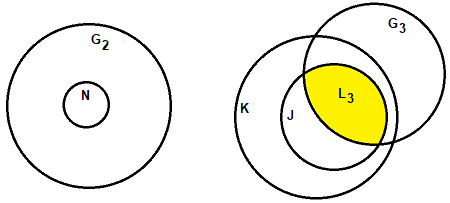
\includegraphics[scale=1]{diagrama_venn}
		\end{center}

		Calcule $L_3 = J \cap G_3 = SO_+(2,1)$.

		Seja $\Psi : \mathbb{R}^3 \rightarrow \mathbb{R}^3 \,; \Psi = \left[ \begin{matrix} a_1 & b_1 & c_1 \\ a_2 & b_2 & c_2 \\ a_3 & b_3 & c_3 \end{matrix} \right]\,$.

		\begin{align*}
		\langle V, V \rangle &= V_1^2 + V_2^2 - V_3^2 \Rightarrow \langle \Psi V, \Psi V \rangle = (a_1 V_1 + b_1 V_2 + c_1 V_3)^2 + (a_2 V_1 + b_2 V_2 + c_2 V_3)^2 - (a_3 V_1 + b_3 V_2 + c_3 V_3)^2 \\
		&= (a_1^2 + a_2^2 - a_3^2) V_1^2 + (b_1^2 + b_2^2 - b_3^2) V_2^2 + (c_1^2 + c_2^2 - c_3^2) V_3^2 + 2 V_1 V_2 (a_1 b_1 + a_2 b_2 - a_3 b_3) + 2 V_1 V_3 (a_1 c_1 + a_2 c_2 - a_3 c_3)  \\
		 &+ 2 V_2 V_3 (b_1 c_1 + b_2 c_2 - b_3 c_3)
		\end{align*}

		\begin{equation*}
		\Psi \in K \Rightarrow
			\left\{\begin{aligned}
			    a_3^2 &= a_1^2 + a_2^2 - 1 \Rightarrow (a_1, a_2, a_3) = (\cosh \mu_1 \cos \lambda_1, \cosh \mu_1 \sin \lambda_1, \sinh \mu_1) \\
			    b_3^2 &= b_1^2 + b_2^2 - 1 \Rightarrow (b_1, b_2, b_3) = (\cosh \mu_2 \cos \lambda_2, \cosh \mu_2 \sin \lambda_2, \sinh \mu_2) \\
			    c_3^2 &= c_1^2 + c_2^2 + 1 \Rightarrow (c_1, c_2, c_3) = (\sinh \varphi \cos \theta, \sinh \varphi \sin \theta, \pm \cosh \varphi) \\
			    a_3 b_3 &= a_1 b_1 + a_2 b_2 \\
			    a_3 c_3 &= a_1 c_1 + a_2 c_2 \\
			    b_3 c_3 &= b_1 c_1 + b_2 c_2
			\end{aligned}
			\right.
		\end{equation*}

		$\Rightarrow {\text{Se }} V_3 \ge 0, \forall\, V_1, V_2 \in \mathbb{R} \Rightarrow a_3 V_1 + b_3 V_2 + c_3 V_3 \ge 0 \Rightarrow \mu_1 \ge 0, \mu_2 \ge 0, \text{sgn } c_3 > 0 $

		\begin{equation*}
		\Psi \in J \Rightarrow
			\left\{\begin{aligned}
				\mu_1, \mu_2 &\ge 0 \\
			    (a_1, a_2, a_3) &= (\cosh \mu_1 \cos \lambda_1, \cosh \mu_1 \sin \lambda_1, \sinh \mu_1) \\
			    (b_1, b_2, b_3) &= (\cosh \mu_2 \cos \lambda_2, \cosh \mu_2 \sin \lambda_2, \sinh \mu_2) \\
			    (c_1, c_2, c_3) &= (\sinh \varphi \cos \theta, \sinh \varphi \sin \theta, \cosh \varphi) \\
			    a_3 b_3 &= a_1 b_1 + a_2 b_2 \\
			    a_3 c_3 &= a_1 c_1 + a_2 c_2 \\
			    b_3 c_3 &= b_1 c_1 + b_2 c_2
			\end{aligned} \Rightarrow \det \left[ \begin{matrix} \cosh \mu_1 \cos \lambda_1 & \cosh \mu_2 \cos \lambda_2 & \sinh \varphi \cos \theta \\ \cosh \mu_1 \sin \lambda_1 & \cosh \mu_2 \sin \lambda_2 & \sinh \varphi \sin \theta \\ \sinh \mu_1 & \sinh \mu_2 & \cosh \varphi \end{matrix} \right] = \,?
			\right.
		\end{equation*}

		\begin{equation*}
		\Psi \in L_3 \Rightarrow
			\left\{\begin{aligned}
				\mu_1, \mu_2 &\ge 0 \\
			    (a_1, a_2, a_3) &= (\cosh \mu_1 \cos \lambda_1, \cosh \mu_1 \sin \lambda_1, \sinh \mu_1) \\
			    (b_1, b_2, b_3) &= (\cosh \mu_2 \cos \lambda_2, \cosh \mu_2 \sin \lambda_2, \sinh \mu_2) \\
			    (c_1, c_2, c_3) &= (\sinh \varphi \cos \theta, \sinh \varphi \sin \theta, \cosh \varphi) \\
			    a_3 b_3 &= a_1 b_1 + a_2 b_2 \\
			    a_3 c_3 &= a_1 c_1 + a_2 c_2 \\
			    b_3 c_3 &= b_1 c_1 + b_2 c_2 \\
			    \det \Psi &= 1\,\,\blacksquare
			\end{aligned}
			\right. \Rightarrow \text{S\~ao 6 vari\'aveis gregas e 4 equa\c{c}\~oes} \Rightarrow \dim L_3 = 2
		\end{equation*}

		\subsection{Verificar que $J$ age em $\mathcal{H}^2$ por isometrias da m\'etrica $m'$ do hiperboloide}
		\begin{flushright}
		\end{flushright}

		Sejam $Q = (r, s, t), P = (\xi, \sigma, \tau) \in \mathcal{H}^2$.

		Pela defini\c{c}\~ao de Hungerford, $J \curvearrowleft \mathcal{H}^2$ se existe produto $\pi : J \times \mathcal{H}^2 \rightarrow \mathcal{H}^2 \,;\, (\Psi, Q) \mapsto \pi(\Psi,Q) = \Psi(Q) = P \in \mathcal{H}^2$

		tal que $\forall \Psi_1, \Psi_2 \in J, \forall Q \in \mathcal{H}^2, I(Q) = Q \wedge (\Psi_1 \Psi_2)(Q) = \Psi_1(\Psi_2 Q)$.

		A \'orbita de $Q$ \'e $J Q = \{ \Psi(Q) \,; \Psi \in J \} $. A a\c{c}\~ao de $J$ \'e transitiva se $J Q = \mathcal{H}^2$, para algum $Q \in \mathcal{H}^2$.

		 $\Psi Q_0 = \left[ \begin{matrix} \cosh \mu_1 \cos \lambda_1 & \cosh \mu_2 \cos \lambda_2 & \sinh \varphi \cos \theta \\ \cosh \mu_1 \sin \lambda_1 & \cosh \mu_2 \sin \lambda_2 & \sinh \varphi \sin \theta \\ \sinh \mu_1 & \sinh \mu_2 & \cosh \varphi \end{matrix} \right] \cdot \left[ \begin{matrix} r_0 \\ s_0 \\ t_0 \end{matrix} \right] = \left[ \begin{matrix} \xi \\ \sigma \\ \tau \end{matrix} \right]$

		 J\'a sabemos que se $Q_0 \in \mathcal{H}^2$, ent\~ao $P \in \mathcal{H}^2$. A volta tamb\'em: $\forall P \in \mathcal{H}^2, \exists Q_0 \in \mathcal{H}^2 \,; Q_0 = \Psi^{-1} P$. Com efeito, matrizes com determinante n\~ao nulo s\~ao invers\'iveis. Provar que $\ker \Psi$ \'e ponto.

		 $\left[ \begin{matrix} \cosh \mu_1 \cos \lambda_1 & \cosh \mu_2 \cos \lambda_2 & \sinh \varphi \cos \theta \\ \cosh \mu_1 \sin \lambda_1 & \cosh \mu_2 \sin \lambda_2 & \sinh \varphi \sin \theta \\ \sinh \mu_1 & \sinh \mu_2 & \cosh \varphi \end{matrix} \right] \cdot \left[ \begin{matrix} r \\ s \\ t \end{matrix} \right] = \left[ \begin{matrix} 0 \\ 0 \\ 0 \end{matrix} \right]$

		 $t = \cfrac{- r \sinh \mu_1 - s \sinh \mu_2}{\cosh \varphi} $

		 $r \cosh \mu_1 \cos \lambda_1 + s \cosh \mu_2 \cos \lambda_2 - r \sinh \mu_1 \tanh \varphi \cos \theta  - s \sinh \mu_2 \tanh \varphi \cos \theta = 0$

		 $\Rightarrow s = - r \cfrac{\cosh \mu_1 \cos \lambda_1 - \sinh \mu_1 \tanh \varphi \cos \theta}{\cosh \mu_2 \cos \lambda_2 - \sinh \mu_2 \tanh \varphi \cos \theta}$

		 $r \cosh \mu_1 \sin \lambda_1 + s \cosh \mu_2 \sin \lambda_2  - r \sinh \mu_1 \tanh \varphi \sin \theta  - s \sinh \mu_2 \tanh \varphi \sin \theta = 0$

		 $\Rightarrow r [\cosh \mu_1 \sin \lambda_1 - \sinh \mu_1 \tanh \varphi \sin \theta] - r \cfrac{\cosh \mu_1 \cos \lambda_1 - \sinh \mu_1 \tanh \varphi \cos \theta}{\cosh \mu_2 \cos \lambda_2 - \sinh \mu_2 \tanh \varphi \cos \theta} [\cosh \mu_2 \sin \lambda_2  - \sinh \mu_2 \tanh \varphi \sin \theta] = 0$

		 $\Rightarrow r = 0 \vee \cfrac{\cosh \mu_1 \sin \lambda_1 - \sinh \mu_1 \tanh \varphi \sin \theta}{\cosh \mu_2 \sin \lambda_2  - \sinh \mu_2 \tanh \varphi \sin \theta} = \cfrac{\cosh \mu_1 \cos \lambda_1 - \sinh \mu_1 \tanh \varphi \cos \theta}{\cosh \mu_2 \cos \lambda_2 - \sinh \mu_2 \tanh \varphi \cos \theta}$

		 $\Rightarrow A/C \cosh \mu_1 - B/C \sinh \mu_1 = D/F \cosh \mu_1 - E/F \sinh \mu_1$

		 $\Rightarrow [A/C - D/F] \cosh \mu_1 = [B/C - E/F] \sinh \mu_1$

		 $\Rightarrow \cfrac{A/C - D/F}{B/C - E/F} = \tanh \mu_1 = \cfrac{AF - CD}{BF - CE} = \cfrac{\sin \lambda_1 [\cos \lambda_2 - \tanh \mu_2 \tanh \varphi \cos \theta] - \cos \lambda_1 [\sin \lambda_2  - \tanh \mu_2 \tanh \varphi \sin \theta]}{\tanh \varphi \sin \theta [\cos \lambda_2 - \tanh \mu_2 \tanh \varphi \cos \theta] - \tanh \varphi \cos \theta [\sin \lambda_2  - \tanh \mu_2 \tanh \varphi \sin \theta]}$

		 $\Rightarrow \tanh \mu_1 \tanh \varphi = \cfrac{\sin \lambda_1 \cos \lambda_2 - \cos \lambda_1 \sin \lambda_2}{ \cos \lambda_2 [ \sin \theta - \cos \theta \tan \lambda_2] } +  \tanh \mu_2 \tanh \varphi \cdot \cfrac{ - \cos \theta \sin \lambda_1  + \sin \theta \cos \lambda_1}{ \cos \lambda_2 [ \sin \theta - \cos \theta \tan \lambda_2] }$

		 \begin{align}
		 \Rightarrow \tanh \mu_1 [ \tan \theta - \tan \lambda_2] = \cfrac{\cos \lambda_1}{\tanh \varphi} \bigg[ \cfrac{\tan \lambda_1 - \tan \lambda_2}{ \cos \theta } +  \tanh \mu_2 \cdot \cfrac{\tan \theta - \tan \lambda_1}{ \cos \lambda_2 } \bigg] \label{igualdade_louca}
		 \end{align}

		\begin{equation*}
		I \in J \Leftrightarrow
			\left\{\begin{aligned}
				\mu_1, \mu_2 &\ge 0 \\
				a_3 &= 0 \Rightarrow \sinh \mu_1 = 0 \Rightarrow \mu_1 = 0 \\
				b_3 &= 0 \Rightarrow \sinh \mu_2 = 0 \Rightarrow \mu_2 = 0 \\
				c_3 &= 1 \Rightarrow \cosh \varphi = 1 \Rightarrow \varphi = 0 \\
			    (c_1, c_2) &= (0, 0) \\
			    (1,0) &= (a_1, a_2) = (\cos \lambda_1, \sin \lambda_1) \Rightarrow \lambda_1 = 0 \\
			    (0,1) &= (b_1, b_2) = (\cos \lambda_2, \sin \lambda_2) \Rightarrow \lambda_2 = \cfrac{\pi}{2} \\
			    0 &= a_1 \cdot 0 + 0 \cdot b_2 \\
			    0 &= a_1 \cdot 0 + a_2 \cdot 0 \\
			    0 &= b_1 \cdot 0 + b_2 \cdot 0
			\end{aligned}
			\right.
		\end{equation*}

		\begin{equation*}
		\Psi Q = P \Leftrightarrow
			\left\{\begin{aligned}
			    \xi &= a_1 r + b_1 s + c_1 t \\
			    \sigma &= a_2 r + b_2 s + c_2 t \\
			    \tau &= a_3 r + b_3 s + c_3 t
			\end{aligned}
			\right. \Rightarrow J\,\Psi = \Psi
		\end{equation*}

		\begin{align*}
		\langle V, V\rangle_Q &= \langle \mathrm{d}\Psi_Q V, \mathrm{d}\Psi_Q V \rangle_{\Psi(Q)} = \langle W, W \rangle_P \Rightarrow W = J\,\Psi\cdot V = \left[ \begin{matrix} \xi_r & \xi_s & \xi_t \\ \sigma_r & \sigma_s & \sigma_t \\ \tau_r & \tau_s & \tau_t \end{matrix} \right] \cdot \left[ \begin{matrix} V_1 \\ V_2 \\ V_3 \end{matrix} \right] \\
		V_1^2 + V_2^2 - V_3^2 &= (\xi_r V_1 + \xi_s V_2 + \xi_t V_3)^2 + (\sigma_r V_1 + \sigma_s V_2 + \sigma_t V_3)^2 - (\tau_r V_1 + \tau_s V_2 + \tau_t V_3)^2 \Rightarrow J\,\Psi \in K, \text{v\'alido }\forall \Psi \in K\,\,\blacksquare
		\end{align*}

		\subsection{$L_2 \cong L_3$}
		\begin{flushright}
		\end{flushright}

		Parece falso. Mostramos que $\dim L_3 = 2 < 3 = \dim L_2$. A n\~ao ser que uma daquelas igualdades seja linearmente dependente.

		\vspace{3mm}

		\begin{align*}
		L_2 = &\left\{ T \circ N = \{ T, -T \} \,; T \bigg\{ \left( \begin{matrix} r^2 & b \\ c & \cfrac{1+ bc}{r^2} \end{matrix} \right) ; r > 0 \,;(r,b,c) \in \mathbb{R}_+ \times \mathbb{R}^2  \bigg\} \right\} \cup \\
		 \cup &\left \{ T \circ N = \{ T, -T \} \,; T \in \bigg\{ \left( \begin{matrix} 0 & b \\ - \cfrac{1}{b} & d \end{matrix} \right) \,; b \ne 0 \,; (b,d) \in \mathbb{R}^2  \bigg\} \right\}
		\end{align*}

		O exerc\'icio pede isomorfismo entre transforma\c{c}\~oes do tipo de M\"obius $(\mathbb{H}^2 \rightarrow \mathbb{H}^2)$ e transforma\c{c}\~oes do tipo $\Psi : \mathcal{H}^2 \rightarrow \mathcal{H}^2$.

		Reveja o diagrama na primeira p\'agina. $\Psi = \pi^{-1} \circ \kappa^{-1} \circ T \circ \kappa \circ \pi$

		$\pi(\xi, \sigma, \tau) = (u, v) \Rightarrow \kappa(\pi(\xi, \sigma, \tau)) = (x, y) \Rightarrow T(\kappa(\pi(\xi, \sigma, \tau))) = (x', y') \Rightarrow \kappa^{-1}(T(\kappa(\pi(\xi, \sigma, \tau)))) = (u', v')$

		$\Rightarrow \pi^{-1}(\kappa^{-1}(T(\kappa(\pi(\xi, \sigma, \tau))))) = (\xi', \sigma', \tau')$

		\vspace{3mm}

		Para simplificar, sejam 6 pontos distintos $Q_3 = (0,0,1), Q_1 = (1,0,\sqrt 2), Q_2 = (0,1,\sqrt 2), P_1, P_2, P_3 \in \mathcal{H}^2$.

		Existe uma \'unica isometria $\Psi$ tal que $\Psi Q_i = P_i$.

		\begin{align*}
		\pi(0,0,1) &= (0, 0) \Rightarrow \kappa(0,0) = (0, 1) \Rightarrow T(0, 1) = \bigg( \cfrac{bd + ac}{c^2 + d^2} , \cfrac{1}{c^2 + d^2} \bigg) \\
		\kappa^{-1}(T(0,1)) &= \cfrac{1}{(bd + ac)^2 + (c^2 + d^2 + 1)^2} [ (2bd + 2ac)(c^2 + d^2), (bd + ac)^2 + 1 - (c^2 + d^2)^2 ] = \bigg( \cfrac{U_3}{D_3}, \cfrac{V_3}{D_3} \bigg) \\
		P_3 &= \cfrac{1}{D^2 - U^2 - V^2} \cdot (2UD, 2VD, D^2 + U^2 + V^2 ) \\
		\pi(1,0,\sqrt 2) &= (\sqrt 2 - 1, 0)\\
		\pi(0,1,\sqrt 2) &= (0, \sqrt 2 - 1)\\
		\kappa(\sqrt 2 - 1, 0) &= \cfrac{\sqrt 2}{2} \cdot (1,1)\\
		\kappa(0, \sqrt 2 - 1) &= (0, 1 + \sqrt 2)\\
		T(\sqrt{0.5}, \sqrt{0.5}) &= \cfrac{1}{2c^2 + 2d^2 + 2cd\sqrt 2} \cdot (2ac + 2ad\sqrt 2 + 2bd - \sqrt 2, \sqrt 2)\\
		T(0, 1 + \sqrt 2) &= \cfrac{1}{d^2 + c^2 (3 + 2\sqrt 2)} \cdot [ bd + ac(3 + 2\sqrt 2) , 1 + \sqrt 2]
		\end{align*}

		\begin{align*}
		\kappa^{-1}(T(\sqrt{0.5}, \sqrt{0.5})) &= \cfrac{1}{(2ac + 2ad\sqrt 2 + 2bd - \sqrt 2)^2 + (\sqrt 2 + 2c^2 + 2d^2 + 2cd\sqrt 2)^2} \cdot \\
		\cdot [ &2(2ac + 2ad\sqrt 2 + 2bd - \sqrt 2)(2c^2 + 2d^2 + 2cd\sqrt 2), \\
		&(2ac + 2ad\sqrt 2 + 2bd - \sqrt 2)^2 + 2 - (2c^2 + 2d^2 + 2cd\sqrt 2)^2 ] = \bigg( \cfrac{U_1}{D_1}, \cfrac{V_1}{D_1} \bigg) \\
		\kappa^{-1}(T(0, 1 + \sqrt 2)) &= \cfrac{1}{[bd + ac(3 + 2\sqrt 2)]^2 + [1 + \sqrt 2 + d^2 + c^2 (3 + 2\sqrt 2)]^2} \{ 2[bd + ac(3 + 2\sqrt 2)][d^2 + c^2 (3 + 2\sqrt 2)], \\
		&[bd + ac(3 + 2\sqrt 2)]^2 + 3 + 2 \sqrt 2 - [d^2 + c^2 (3 + 2\sqrt 2)]^2 \} = \bigg( \cfrac{U_2}{D_2}, \cfrac{V_2}{D_2} \bigg) \\
		P_1 &= \cfrac{1}{D^2 - U^2 - V^2} \cdot (2UD, 2VD, D^2 + U^2 + V^2 ) \\
		P_2 &= \cfrac{1}{D^2 - U^2 - V^2} \cdot (2UD, 2VD, D^2 + U^2 + V^2 ) \\
		\text{Associamos }&\Psi\text{ com a base }B = \left[ \begin{matrix} 1 & 0 & 0 \\ 0 & 1 & 0 \\ \sqrt 2 & \sqrt 2 & 1 \end{matrix} \right] \Rightarrow [\Psi]_B = \left[ \begin{matrix} P_1^1 & P_2^1 & P_3^1 \\ P_1^2 & P_2^2 & P_3^2 \\ P_1^3 & P_2^3 & P_3^3 \end{matrix} \right]
		\end{align*}

		Ser\'a que $\langle \Psi Q, \Psi Q \rangle = \langle Q, Q \rangle$? Ser\'a que $\det \Psi = 1$? Engaveto sem fazer as contas, acreditando que para todo $\kappa(a,b,c,d)$ existe $\Psi$ e que para todo $\Psi$, existe $\kappa$, perfazendo uma bije\c{c}\~ao desejada entre $L_2$ e $L_3$. Sabemos que: nem toda bije\c{c}\~ao \'e um isomorfismo.

		Para fechar com chave de ouro, tenha f\'e em que a equa\c{c}\~ao (\ref{igualdade_louca}) \'e falsa para todo $\lambda_1, \lambda_2, \mu_1, \mu_2, \theta, \varphi$.

		\vspace{120mm}

		\subsection{$\Phi = \{ T : \mathbb{H}^2 \rightarrow \mathbb{H}^2 \,; T(z) = \cfrac{az + b}{cz + d} \,; ad - bc = 1 \,; z \in \mathbb{H}^2 \,; a,b,c,d \in \mathbb{R} \}$ \'e um grupo.}
		\begin{flushright}
		\end{flushright}

		Fechamento: se $U(z) = \cfrac{pz + q}{rz + s} \,; ps - qr = 1 \,; p,q,r,s \in \mathbb{R}$ Ent\~ao $U \circ T \in \Phi$.

		Demo: $U(T(z)) = \cfrac{pT(z) + q}{rT(z) + s} = \cfrac{p(az + b) + q(cz + d)}{r(az + b) + s(cz + d)} = \cfrac{(ap + cq) z + bp + dq}{(ar + cs)z + br + ds} = \cfrac{a'z + b'}{c'z + d'} $

		Queremos mostrar que $a'd' = b'c' + 1$

		$\cancel{apbr} + apds + cqbr + \cancel{cqds} = \cancel{bpar} + bpcs + dqar + \cancel{dqcs} + 1$

		$ps(ad - bc) + qr(bc - ad) = 1 = (ad - bc)(ps - qr) = 1 \cdot 1$

		Associatividade \'e imediato: $T,U,V : \mathbb{C} \rightarrow \mathbb{C}$ Ent\~ao $(T \circ U) \circ V = T \circ (U \circ V)$.

		Elemento neutro: $\exists I \in \Phi \,; T \circ I = I \circ T = T$

		Demo: Basta definir $I(z) = z$ quando $(a,b,c,d) = (1,0,0,1)$.

		$T(I(z)) = T(z) = w$

		$I(T(z)) = I(w) = w = T(z)$

		Elemento inverso: $\exists T^{-1} \in \Phi \,; T \circ T^{-1} = T^{-1} \circ T = I$

		Demo: Seja $T^{-1}(z) = \cfrac{pz + q}{rz + s}$

		\begin{equation*}
			\left.\begin{aligned}
			    ap + cq &= 1    \\
			    bp + dq &= 0 \Rightarrow q = -\cfrac{bp}{d} \,\,\textbf{(i)}  \\
			    ar + cs &= 0 \Rightarrow s = -\cfrac{ar}{c} \,\,\textbf{(ii)}   \\
			    br + ds &= 1 \,\,\textbf{(iii)}
			\end{aligned}
			\right\} \Rightarrow ap - \cfrac{bcp}{d} = 1 \Rightarrow p = \cfrac{d}{\cancel{ad - bc}} = d
		\end{equation*}

		$\textbf{(i)} \Rightarrow q = -b$

		$\textbf{(iii)} \Rightarrow br - \cfrac{adr}{c} = 1 \Rightarrow r = -\cfrac{c}{\cancel{ad - bc}} = -c$

		$\textbf{(ii)} \Rightarrow s = a$

		Logo, $T^{-1}(z) = \cfrac{dz - b}{-cz + a}\,$. Portanto, $(\Phi, \circ)$ \'e grupo. $\,\,\blacksquare$

\section{Toro}
		\begin{flushright}
		\end{flushright}

		$0 < r < R\,;\,t \in I \stackrel{\gamma}{\longrightarrow} (\lambda,\mu) \in U \stackrel{\varphi}{\longrightarrow} p = (x,y,z) \in T^2$.

		$\varphi(\lambda, \mu) = \left[ \begin{matrix} (R + r \cos \lambda) \cos \mu \\ (R + r \cos \lambda) \sin \mu \\ r \sin \lambda \end{matrix} \right] \Rightarrow \varphi_\lambda = \left[ \begin{matrix} - r \sin \lambda \cos \mu \\ - r \sin \lambda \sin \mu \\ r \cos \lambda \end{matrix} \right] \Rightarrow \varphi_\mu = \left[ \begin{matrix} (R + r \cos \lambda) \cos \mu \\ (R + r \cos \lambda) \sin \mu \\ r \sin \lambda \end{matrix} \right]$

		$x^2 + y^2 = (R + r \cos \lambda)^2 \Rightarrow - R \pm \sqrt{x^2 + y^2} = r \cos \lambda \Rightarrow (- R \pm \sqrt{x^2 + y^2})^2 + z^2 = r^2$

		$\Rightarrow R^2 + x^2 + y^2 + z^2 \mp 2 R \sqrt{x^2 + y^2} = r^2 \therefore (x^2 + y^2 + z^2 + R^2 - r^2)^2 = 4R^2 (x^2 + y^2)$

		$g_{ij}$ vem da equa\c{c}\~ao 2.3 na p. 46.

		$\Gamma_{ij}^k$ vem da equa\c{c}\~ao 3.19 na p. 72. Proposi\c{c}\~ao 3.14: Se a conex\~ao $\nabla$ \'e sim\'etrica, ent\~ao $\Gamma_{ij}^k = \Gamma_{ji}^k$.

		Defini\c{c}\~ao 5.1 na p. 101: Endomorfismo curvatura de $M$ \'e $R : \mathcal{T}(M) \times \mathcal{T}(M) \times \mathcal{T}(M) \rightarrow \mathcal{T}(M)$

		$(X, Y, Z) \mapsto R(X,Y)Z = \nabla_X \nabla_Y Z - \nabla_Y \nabla_X Z - \nabla_{[X,Y]} Z$

		\begin{align*}
		\text{Equa\c{c}\~ao 5.23 na p. 109 } \Leftrightarrow R = &\sum_i \sum_j \sum_k \sum_\ell R_{ijk}^\ell \mathrm{d}x^i \otimes \mathrm{d}x^j \otimes \mathrm{d}x^k \otimes \partial_\ell \\
		\text{Equa\c{c}\~ao 5.8 na p. 103 } \Leftrightarrow R(X,Y)Z = &\sum_i \sum_j \sum_k \sum_\ell R_{ijk}^\ell X^i Y^j Z^k \partial_\ell
		\end{align*}

		A f\'ormula dos $R_{ijk}^\ell$ vem da proposi\c{c}\~ao 5.3 na p. 102.

		p. 105, Proposi\c{c}\~ao 5.6: $R_{ijk}^\ell = -R_{jik}^\ell \Rightarrow R_{iik}^\ell = 0$.

		Defini\c{c}\~ao 5.12 na p. 109: Tensor curvatura de $M$ \'e $R : \mathcal{T}(M) \times \mathcal{T}(M) \times \mathcal{T}(M) \times \mathcal{T}(M) \rightarrow C^\infty(M)$

		$(X, Y, Z, W) \mapsto \langle R(X,Y)Z, W \rangle$

		\begin{align*}
		R = \sum_i \sum_j \sum_k \sum_\ell R_{ijk\ell} \mathrm{d}x^i \otimes \mathrm{d}x^j \otimes \mathrm{d}x^k \otimes \mathrm{d}x^\ell
		\end{align*}

		As componentes do tensor curvatura v\^em da proposi\c{c}\~ao 5.13 na p. 109

		Proposi\c{c}\~ao 5.14 na p. 110: $- R_{ij\ell k} = R_{ijk\ell} = - R_{jik\ell}\,; R_{ijk\ell} = R_{k\ell ij}$

		Corol\'ario 5.15 na p. 111: $R_{iik\ell} = 0 = R_{ijkk}$

		Defini\c{c}\~ao 5.20 na p. 118: Tensor curvatura de Ricci de $M$ \'e $R_{ij} = R_{1ij}^1 + \cdots + R_{nij}^n$

		Proposi\c{c}\~ao 5.21: $R_{ij} = R_{ji}$

		\begin{align*}
		&\text{Def. 5.22: Curvatura escalar de } M \text{ \'e } S : M \rightarrow \mathbb{R}\,; S = \text{tr}_g \text{Ric} = \sum_i \sum_j g^{ij} R_{ij}. \\
		&\text{Def. 5.28 na p. 121: } \sigma \text{ \'e plano de } T_pM, \{X, Y \} \text{ \'e base de } \sigma, \text{ Curvatura seccional de }M, \sigma \text{ \'e } K(X,Y) = \cfrac{R(X,Y,Y,X)}{\Vert X \Vert^2 \Vert Y \Vert^2 - \langle X, Y \rangle^2} \\
		&\text{Equa\c{c}\~ao 5.44 na p. 124: }S = \sum_{i \ne j} K(E_i, E_j)
		\end{align*}

		\begin{align*}
		g_{11} &= \langle \varphi_\lambda, \varphi_\lambda \rangle = r^2 \cdot \cancel{(\sin^2 \lambda + \cos^2 \lambda)} \\
		g_{12} &= g_{21} = \langle \varphi_\lambda, \varphi_\mu \rangle = r (R + r \cos \lambda) \sin \mu \cos \mu \sin \lambda (1 - 1) = 0 \\
		g_{22} &= \langle \varphi_\mu, \varphi_\mu \rangle = (R + r \cos \lambda)^2 \cdot \cancel{(\sin^2 \mu + \cos^2 \mu)} \\
		G &= \left[ \begin{matrix} r^2 & 0 \\ 0 & (R + r \cos \lambda)^2 \end{matrix} \right] \Rightarrow G^{-1} = \left[ \begin{matrix} \cfrac{1}{r^2} & 0 \\ 0 & \cfrac{1}{(R + r \cos \lambda)^2} \end{matrix} \right] \\
		\Gamma_{11}^1 &= \cfrac{1}{2} \sum_{m = 1}^2 (\partial_1 g_{1m} + \partial_1 g_{1m} - \partial_m g_{11}) g^{m1} = 0 \\
		\Gamma_{11}^2 &= \cfrac{1}{2} \sum_m (\partial_1 g_{2m} + \cancel{\partial_2 g_{1m}} - \partial_m g_{12}) g^{m1} = \cfrac{1}{2} (\partial_1 g_{21} - \partial_1 g_{12}) g^{11} = 0 \\
		\Gamma_{12}^1 &= \cfrac{1}{2} \sum_m (\partial_1 g_{2m} + \cancel{\partial_2 g_{1m}} - \partial_m g_{12}) g^{m1} = \cfrac{1}{2} \cdot (\partial_1 g_{21} - \partial_1 g_{12}) g^{11} = 0 \\
		\Gamma_{12}^2 &= \Gamma_{21}^2 = \cfrac{1}{2} \sum_m (\partial_1 g_{2m} + \partial_2 g_{1m} - \partial_m g_{12}) g^{m2} = \cfrac{1}{2} (\partial_1 g_{22} + \partial_2 g_{12} - \partial_2 g_{12}) g^{22} = \cfrac{- r \sin \lambda}{R + r \cos \lambda} \\
		\Gamma_{22}^1 &= \cfrac{1}{2} \sum_m (\cancel{\partial_2 g_{2m}} + \cancel{\partial_2 g_{2m}} - \partial_m g_{22}) g^{m1} = r^3 \sin \lambda (R + r \cos \lambda) \\
		\Gamma_{22}^2 &= \cfrac{1}{2} \sum_m (\cancel{\partial_2 g_{2m}} + \cancel{\partial_2 g_{2m}} - \partial_m g_{22}) g^{m2} = 0 \\
		R_{111}^\ell &= \sum_m (\Gamma_{11}^m \Gamma_{1m}^\ell - \Gamma_{11}^m \Gamma_{1m}^\ell) + \cfrac{\partial \Gamma_{11}^\ell}{\partial x^1} - \cfrac{\partial \Gamma_{11}^\ell}{\partial x^1} = 0 \Rightarrow R_{112}^\ell = \sum_m (\Gamma_{12}^m \Gamma_{1m}^\ell - \Gamma_{12}^m \Gamma_{1m}^\ell) + \cfrac{\partial \Gamma_{12}^\ell}{\partial x^1} - \cfrac{\partial \Gamma_{12}^\ell}{\partial x^1} = 0 \\
		R_{122}^\ell &= \sum_m (\Gamma_{22}^m \Gamma_{1m}^\ell - \Gamma_{12}^m \Gamma_{2m}^\ell) + \cfrac{\partial \Gamma_{22}^\ell}{\partial x^1} - \cancel{\cfrac{\partial \Gamma_{12}^\ell}{\partial x^2}} \\
		R_{122}^1 &= \Gamma_{22}^1 \cancel{\Gamma_{11}^\ell} - \Gamma_{12}^1 \cancel{\Gamma_{21}^\ell} + \cancel{\Gamma_{22}^2} \Gamma_{12}^\ell - \Gamma_{12}^2 \Gamma_{22}^\ell + r^3 [ \cos \lambda (R + r \cos \lambda) + \sin \lambda (-r \sin \lambda) ] = r^3 R \cos \lambda + r^4 \cos^2 \lambda - 2 r^4 \sin^2 \lambda \\
		R_{122}^2 &= 0 - 0 + 0 - 0 + 0 = 0 \\
		R_{121}^\ell &= \sum_m (\Gamma_{21}^m \Gamma_{1m}^\ell - \Gamma_{11}^m \Gamma_{2m}^\ell) + \cfrac{\partial \Gamma_{21}^\ell}{\partial x^1} - \cancel{\cfrac{\partial \Gamma_{11}^\ell}{\partial x^2}} \Rightarrow R_{121}^1 = \cancel{\Gamma_{21}^1 \Gamma_{11}^\ell} - \cancel{\Gamma_{11}^1 \Gamma_{21}^\ell} + \Gamma_{21}^2 \Gamma_{12}^\ell - \cancel{\Gamma_{11}^2 \Gamma_{22}^\ell} + 0 = 0 \\
		R_{121}^2 &= \cfrac{r^2 \sin^2 \lambda - r^2 \sin^2 \lambda}{(R + r \cos \lambda)^2} - r \cos \lambda (R + r \cos \lambda)^{1 - 2} = \cfrac{-r \cos \lambda}{R + r \cos \lambda} \\
		R_{211}^\ell &= - R_{121}^\ell \Rightarrow R_{211}^1 = 0 \Rightarrow R_{211}^2 = \cfrac{r \cos \lambda}{R + r \cos \lambda} \\
		R_{212}^1 &= - R_{122}^1 = - r^3 R \cos \lambda - r^4 \cos^2 \lambda + 2 r^4 \sin^2 \lambda \Rightarrow R_{212}^2 = - R_{122}^2 = 0 \Rightarrow R_{221}^\ell = 0 \Rightarrow R_{222}^\ell = 0 \\
		R_{ijk\ell} &= g_{1\ell} R_{ijk}^1 + g_{2\ell} R_{ijk}^2 \\
		i = j \Rightarrow 0 &= R_{1111} = R_{1112} = R_{1121} = R_{1122} = R_{2211} = R_{2212} = R_{2221} = R_{2222} \\
		k = \ell \Rightarrow 0 &= R_{1211} = R_{1222} = R_{2111} = R_{2122} \\
		R_{1212} &= g_{12} \cancel{R_{121}^1} + g_{22} R_{121}^2 = - r \cos \lambda (R + r \cos \lambda) = A(\lambda) \Rightarrow R_{1221} = - A(\lambda) \Rightarrow R_{2121} = A(\lambda) \Rightarrow R_{2112} = - A(\lambda)
		\end{align*}

		\begin{align*}
		R_{11} &= \cancel{R_{111}^1} + R_{211}^2 = \cfrac{-r^2 \sin^2 \lambda}{(R + r \cos \lambda)^2} \\
		R_{12} &= R_{21} = \cancel{R_{112}^1} + R_{212}^2 = 0 \\
		R_{22} &= R_{122}^1 + \cancel{R_{222}^2} = r^3 R \cos \lambda + r^4 \cos^2 \lambda - 2 r^4 \sin^2 \lambda
		\end{align*}

		Seja $\{ E_1, E_2 \}$ base ortonormal para $T_pT^2$

		$S = \text{tr}_g \text{Ric} = g^{11} R_{11} + g^{12} \cancel{R_{12}} + g^{21} \cancel{R_{21}} + g^{22} R_{22}$

		$S = \cfrac{R_{11}}{r^2} + \cfrac{R_{22}}{(R + r \cos \lambda)^2} = \cfrac{r^3 \cos \lambda}{R + r \cos \lambda} + \cfrac{- \sin^2 \lambda - 2 r^4 \sin^2 \lambda}{(R + r \cos \lambda)^2}$ = curvatura escalar

		Pela equa\c{c}\~ao 5.45, $S(p) = K(E_1, E_2) + K(E_2, E_1) = 2 K(p)$

		$K(p) = \cfrac{1}{2} \cdot S(p) = $ curvatura seccional.

		\vspace{3mm}

		Como vimos no exerc\'icio 1,

		\begin{align}
		  \cfrac{\mathrm{d}^2 \gamma^k}{\mathrm{d} t^2} + \sum_i \sum_j \Gamma_{ij}^k \cdot \cfrac{\mathrm{d} \gamma^i}{\mathrm{d} t} \cdot \cfrac{\mathrm{d} \gamma^j}{\mathrm{d} t} &= 0, \forall k \\
		  \text{Denotamos } \gamma^k_{tt} + \sum_i \sum_j \Gamma_{ij}^k \cdot \gamma^i_t \cdot \gamma^j_t &= 0, \forall k \label{geodesica_tt}
		\end{align}

		Equa\c{c}\~oes geod\'esicas do toro:

		\begin{equation*}
			(\ref{geodesica_tt}) \Rightarrow \left\{\begin{aligned}
			    0 &= \lambda_{tt} + \cancel{\Gamma_{11}^1} \lambda_t^2 + \cancel{\Gamma_{12}^1} \lambda_t \mu_t + \cancel{\Gamma_{21}^1} \mu_t \lambda_t + \Gamma_{22}^1 \mu_t^2 \\
			    0 &= \mu_{tt} + \cancel{\Gamma_{11}^2} \lambda_t^2 + (\Gamma_{12}^2 + \Gamma_{21}^2) \lambda_t \mu_t + \cancel{\Gamma_{22}^2} \mu_t^2
			\end{aligned}
			\right.
		\end{equation*}

		\begin{equation*}
			\left\{\begin{aligned}
			    \lambda_{tt} + r^3 \sin \lambda (R + r \cos \lambda) \mu_t^2 &= 0 \,\,\textbf{(i)} \\
			    \mu_{tt} - \cfrac{2r \sin \lambda}{R + r \cos \lambda} \lambda_t \mu_t &= 0 \,\,\textbf{(ii)}
			\end{aligned}
			\right.
		\end{equation*}

		Equadores interno e externo s\~ao geod\'esicas: $z = 0 \Rightarrow \sin \lambda = 0 \Rightarrow \lambda(t) \equiv 0 \vee \lambda(t) \equiv \pi$.

		\begin{equation*}
		  \lambda(t) \equiv 0 \Rightarrow
			\left\{\begin{aligned}
			    0_{tt} + \sin 0 &= 0, \forall \mu \\
			    \mu_{tt} - \sin 0 &= 0 \Rightarrow \mu(t) = c_1 t + c_2 \,; c_i \in \mathbb{R}
			\end{aligned}
			\right.
		\end{equation*}

		\begin{equation*}
		  \lambda(t) \equiv \pi \Rightarrow
			\left\{\begin{aligned}
			    \pi_{tt} + \sin \pi &= 0, \forall \mu \\
			    \mu_{tt} - \sin \pi &= 0 \Rightarrow \mu(t) = c_3 t + c_4
			\end{aligned}
			\right.
		\end{equation*}

		Meridianos s\~ao geod\'esicas: $\{ z = z_0 \in \mathbb{R} \} \perp \{ ax + by = 0\,; a, b \in \mathbb{R} \} \Rightarrow x = 0 \vee y = x \tan k, k \in \mathbb{R}$

		$\Rightarrow \cancel{(R + r \cos \lambda)} \sin \mu = \cancel{(R + r \cos \lambda)} \cos \mu \tan k  \Rightarrow \tan \mu = \tan k \Rightarrow \mu(t) \equiv k$.

		\begin{equation*}
		  \mu(t) \equiv k \Rightarrow
			\left\{\begin{aligned}
			    \lambda_{tt} + k_t^2 &= 0 \Rightarrow \lambda(t) = c_5 t + c_6 \\
			    k_{tt} - k_t &= 0, \forall \lambda
			\end{aligned}
			\right.
		\end{equation*}

		Procuramos solu\c{c}\~oes de \textbf{(i)} e \textbf{(ii)} al\'em de equadores e meridianos.

		\vspace{3mm}

		$w = R + r \cos \lambda \Rightarrow w_t = -r \lambda_t \sin \lambda$

		\textbf{(ii)} $\Rightarrow \mu_{tt} + \cfrac{\mu_t w_t}{w} \cdot 2 = 0 \Rightarrow \cfrac{\mu_{tt}}{\mu_t} = -2 \cdot \cfrac{w_t}{w}\,$. Integrando, $\log \mu_t = \log w^{-2} + \log c_7 \Rightarrow \mu_t = \cfrac{c_7}{w^2} = \cfrac{c_7}{(R + r \cos \lambda)^2}$

		\textbf{(i)} $\Rightarrow \lambda_{tt} + r^3 \sin \lambda (R + r \cos \lambda)^{1 - 4} c_7^2 = 0 \Rightarrow \lambda_{tt} \lambda_t - \cfrac{c_7^2}{w^3} \cdot w_t \cdot r^2 = 0 \Rightarrow \cfrac{1}{2} \cfrac{\mathrm{d}}{\mathrm{d}t} (\lambda_t^2) = c_7^2 r^2 \cdot \cfrac{w_t}{w^3}$

		Integrando, $\cfrac{1}{2} \cdot \lambda_t^2 = - \cfrac{c_7^2 r^2}{2w^2} + c_8$. Utilizamos a propriedade da geod\'esica: $\mu_t^2 + \lambda_t^2 = c_9 \Rightarrow \cfrac{c_7^2}{w^4} - \cfrac{c_7^2 r^2}{w^2} + 2c_8 = c_9$

		$\Rightarrow \cfrac{1}{w^4} - \cfrac{r^2}{w^2} = \cfrac{c_9 - 2c_8}{c_7^2} = c_{10} \Rightarrow c_{10} w^4 + r^2 w^2 - 1 = 0 \Rightarrow w^2(r) = \cfrac{-r^2 \pm \sqrt{r^4 + 4 c_{10}}}{2c_{10}}$

		\begin{equation*}
			\left\{\begin{aligned}
			    \mu_t &= \cfrac{c_7}{w^2} = f(r) \Rightarrow \mu(t) = f(r) t + \mu_0 \\
			    \lambda_t &= \pm \sqrt{2c_8 - \cfrac{c_7 r^2}{w^2}} = \pm g(r) \Rightarrow \lambda(t) = \pm g(r) t + \lambda_0
			\end{aligned}
			\right. \Rightarrow (\lambda, \mu) = t \cdot (v_1, v_2) + (\lambda_0, \mu_0) \in \mathbb{R}^2
		\end{equation*}

		$v_1 = \pm \sqrt{2c_8 - \cfrac{2c_7 c_{10} r^2}{-r^2 \pm \sqrt{r^4 + 4 c_{10}}}} = \pm \sqrt{\cfrac{4c_8 + c_7 r^2 \bigg(-r^2 \mp \sqrt{r^4 + 4 \cfrac{c_9 - 2c_8}{c_7^2}}\bigg)}{2}} = \pm \sqrt{\cfrac{4c_8 - c_7 r^4 \mp r^2 \sqrt{c_7^2 r^4 + 4 c_9 - 8c_8}}{2}}$

		$v_2 = \cfrac{2c_7c_{10}}{-r^2 \pm \sqrt{r^4 + 4 c_{10}}} = \cfrac{c_7 r^2 \pm \sqrt{c_7^2 r^4 + 4 c_9 - 8c_8}}{2} \Rightarrow v_1 = \pm \sqrt{2c_8 - r^2 v_2} \therefore v_2 = \cfrac{2c_8 - v_1^2}{r^2}$

		\vspace{3mm}

		Portanto, imagens de retas por $\varphi$ s\~ao geod\'esicas. Retas verticais, equadores. Retas horizontais, meridianos. Retas diagonais:

		$\varphi(\lambda_0 + v_1 t, \mu_0 + v_2 t) = \left[ \begin{matrix} [R + r \cos (\lambda_0 + v_1 t)] \cos (\mu_0 + v_2 t) \\ [R + r \cos (\lambda_0 + v_1 t)] \sin (\mu_0 + v_2 t) \\ r \sin (\lambda_0 + v_1 t) \end{matrix} \right] = \gamma(t)\,\,\blacksquare$

		Se algu\'em conferiu, me mande. Eu tenho f\'e que as geod\'esicas no toro ou s\~ao peri\'odicas de per\'iodo fra\c{c}\~ao vezes $\pi$, ou s\~ao densas no toro.

		Certa vez, perguntei no math.stack.exchange.com se algu\'em tinha uma prova direta de que, se eu pego uma \'unica geod\'esica densa $\gamma$, um ponto $p \notin \gamma$, considero uma bolinha aberta $U = B(p, \epsilon) \subset \mathbb{R}^3$, precisamos encontrar algum ponto $q \in \gamma \cap U$. Existem infinitos pontos desses, por f\'e na densidade de $\gamma$. Mas estou sem resposta at\'e hoje. A pergunta se perdeu por excesso de informa\c{c}\~oes na nuvem.

	\section{Quest\~ao de Lee 5.4, p. 71}
		\begin{flushright}
		\end{flushright}

		Verificar que $\kappa$(c\'irculo ortogonal, reta que cont\'em origem) = $\{ x = x_0 \} \cup \{ (x - x_0)^2 + y^2 = R^2 \}$

		\begin{align*}
		x = x_0 &\Rightarrow (y + 1)^2 = 2x_0/u - x_0^2 \Rightarrow y = -1 + \epsilon \sqrt{2x_0/u - x_0^2} \\
		x_0^2 v &+ (y + 1)^2 v = x_0^2 + y^2 - 1 \Rightarrow 2x_0 v/u = 2x_0/u - 2\epsilon \sqrt{2x_0/u - x_0^2} \\
		&\Rightarrow (v - 1)^2 = 2u/x_0 - u^2 \Rightarrow (u - 1/x_0)^2 + (v - 1)^2 = 1/x_0^2, \text{ caso } x_0 \ne 0 \\
		x_0 = 0 &\Rightarrow u = 0, -1 < v(t) < 1\\
		0 < t < \pi &\Rightarrow (x, y) = f(t) = (R \cos t + x_0, R \sin t)
		\end{align*}

		Sejam 6 pontos distintos quaisquer $z_1 = f(\pi/6), z_2 = f(\pi/3), z_3 = f(\pi/2) \in \mathbb{H}^2, w_1, w_2, w_3 \in B^2$.

		Existe uma \'unica transformada de Cayley $\kappa$ tal que $\kappa(w_i) = z_i, i \in \{ 1, 2, 3 \} \Rightarrow \kappa(u_i, v_i) = (x_i, y_i)$.

		$z_1 = (R \sqrt{3}/2 + x_0, R/2)$

		$z_2 = (R/2 + x_0, R \sqrt{3}/2)$

		$z_3 = (x_0, R)$

		$\kappa^{-1}(z_1) = 1 / [(R\sqrt{3}/2 + x_0)^2 + (R/2 + 1)^2] \cdot [2(R\sqrt{3}/2 + x_0), (R\sqrt{3}/2 + x_0)^2 + R^2/4 - 1]$

		$\kappa^{-1}(z_2) = 1 / [(R/2 + x_0)^2 + (R\sqrt{3}/2 + 1)^2] \cdot [2(R/2 + x_0), (R/2 + x_0)^2 + 3 R^2/4 - 1]$

		$\kappa^{-1}(z_3) = 1 / [x_0^2 + (R + 1)^2] \cdot [2x_0, x_0^2 + R^2 - 1]$

		Ou $w_1, w_2, w_3$ est\~ao alinhados, ou formam um c\'irculo simples euclideano.

		Determinar $t$ tal que $w_1 = w_3 + (w_2 - w_3)t$.

		$u_1 = u_3 + (u_2 - u_3) t$

		$v_1 = v_3 + (v_2 - v_3) t$

		$t = \cfrac{u_1 - u_3}{u_2 - u_3} = \cfrac{v_1 - v_3}{v_2 - v_3}$

		\vspace{3mm}

		Determinar $u,v,r$ no sistema abaixo.

		$(u_1 - u)^2 + (v_1 - v)^2 = r^2$

		$(u_2 - u)^2 + (v_2 - v)^2 = r^2$

		$(u_3 - u)^2 + (v_3 - v)^2 = r^2$

		$(u_1 - u)^2 + (v_1 - v)^2 = (u_2 - u)^2 + (v_2 - v)^2$

		$u_1^2 - 2u_1 u + u^2 + v_1^2 - 2v_1 v + v^2 = u_2^2 - 2u_2 u + u^2 + v_2^2 - 2v_2 v + v^2$

		$\cfrac{u_1^2 + v_1^2 - u_2^2 - v_2^2 + (2u_2 - 2u_1) u}{2v_1 - 2v_2} = v(u) = \cfrac{au + b}{d}$

		$r^2(u) = (u_1 - u)^2 + \bigg(v_1 - \cfrac{u_1^2 + v_1^2 - u_2^2 - v_2^2 + (2u_2 - 2u_1) u}{2v_1 - 2v_2}\bigg)^2 $

		$(u_3 - u)^2 + \bigg(v_3 - \cfrac{au + b}{d} \bigg)^2 = (u_1 - u)^2 + \bigg(v_1 - \cfrac{au + b}{d}\bigg)^2 $

		$u_3^2 - 2 u_3 u + u^2 + v_3^2 - 2 v_3 \cfrac{au + b}{d} + \cfrac{(au+b)^2}{d^2} = u_1^2 - 2 u_1 u + u^2 + v_1^2 - 2 v_1 \cfrac{au + b}{d} + \cfrac{(au+b)^2}{d^2}$

		$u = \cfrac{(u_1^2 + v_1^2 - u_3^2 - v_3^2)d + (2 v_3 - 2 v_1) b}{(2 u_1 - 2 u_3)d + (2 v_1 - 2 v_3)a}$

		$u = \cfrac{(u_1^2 + v_1^2 - u_3^2 - v_3^2)(v_1 - v_2) + (v_3 - v_1) (u_1^2 + v_1^2 - u_2^2 - v_2^2)}{(u_1 - u_3)(2v_1 - 2v_2) + (2 v_1 - 2 v_3)(u_2 - u_1)}$

		Engaveto sem provar que a reta passa pela origem e que o c\'irculo \'e ortogonal.

		Determinar $t$ tal que $0 = w_3 + (w_2 - w_3)t$.

		$0 = u_3 + (u_2 - u_3) t$

		$0 = v_3 + (v_2 - v_3) t$

		$t = \cfrac{- u_3}{u_2 - u_3} = \cfrac{- v_3}{v_2 - v_3}$

		Essa igualdade \'e pura f\'e. Fora da caridade n\~ao h\'a salva\c{c}\~ao. Em toda reprodu\c{c}\~ao biol\'ogica h\'a Evolu\c{c}\~ao.

\end{document}
